% Detailed evaluation diagnostics displaced from Chapter 5 by the 2026-07 restructure.
% Refreshed items are sourced from MLP/eval_pipeline run evalrun_20260709_223144_thesis_full_fullclean_bootstrap_fast_20260709_223142;
% archived items are retained verbatim from the pre-restructure chapter (2026-05/06 artifact bundles).
\section{Detailed Evaluation Diagnostics}
\label{app:evaluation-diagnostics}

This appendix collects the detailed diagnostic tables and figures that supported
the pre-restructure version of Chapter~5. The main text now reports the
condensed verdicts; the material below preserves the full evidence trail. Two
provenance classes are kept apart throughout: \emph{refreshed} items are
regenerated by the evaluation pipeline (run
\texttt{evalrun\_\allowbreak{}20260709\_\allowbreak{}223144}) on the QC-gated
dataset root, while \emph{archived} items are retained verbatim from the
earlier thesis artifact bundles and are labeled as such.

\subsection{Archive Scale and Fitted-Target Example}

The extraction and fitting workflow generated 295 cleaned fitted trajectory
files across the processed campaign archives after converting a high-throughput
Mie video archive into structured CSV/JSON tables, checkpoints, fitted targets,
model artifacts, and diagnostic plots. Across the broader archive, the workflow
covers 9 nozzles, 266 condition subfolders, and 2,992 recording files; its
practical value lies in making terabyte-scale raw optical inputs reproducible
and auditable rather than leaving them as isolated post-processing products.
Figure~\ref{fig:clean-fit-example} shows a representative fitted-target
example: the cleaned curves retain the plume-to-plume variation, while the
fitted trajectories provide a smooth and censoring-aware target that remains
faithful to the observed liquid-phase envelope.

\begin{figure}[t]
\centering
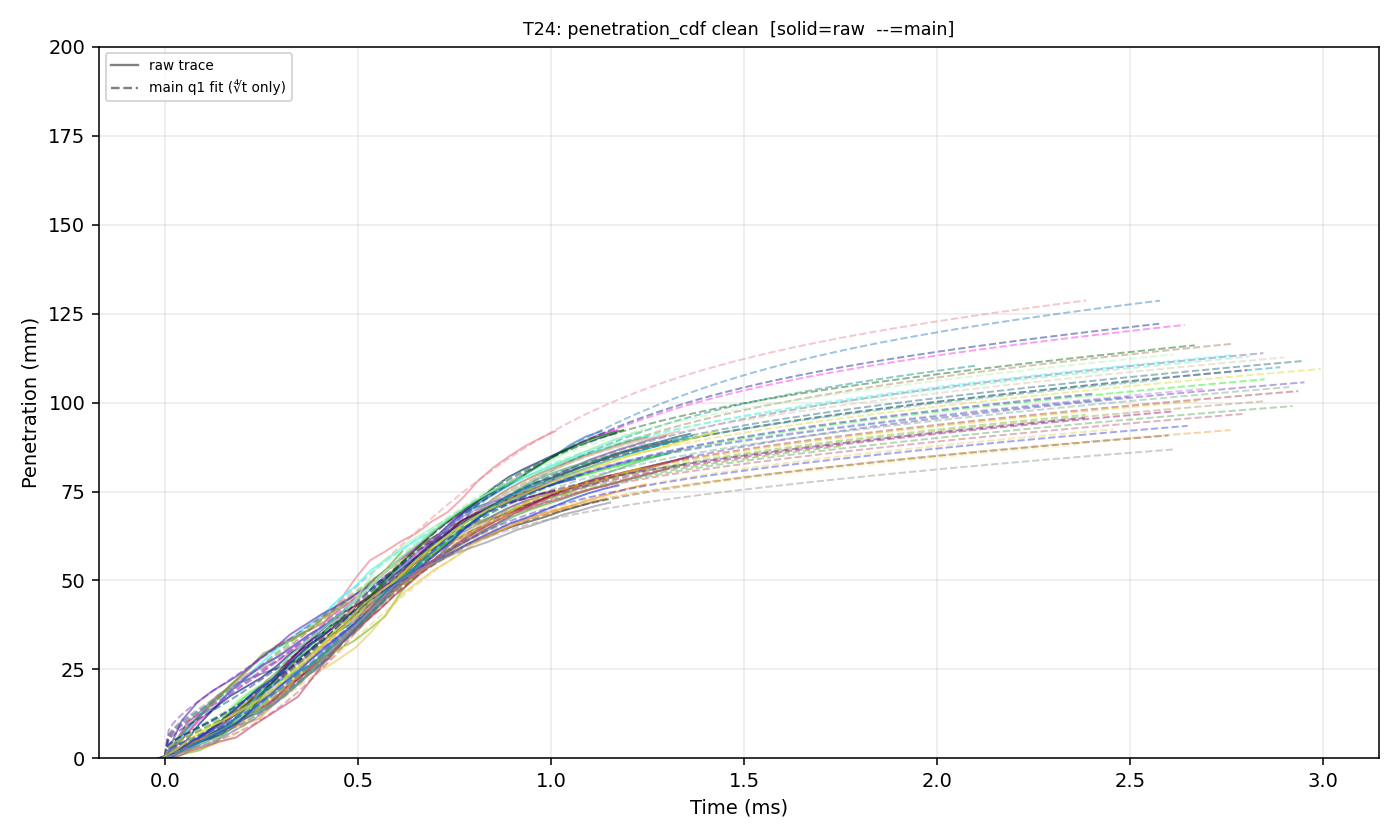
\includegraphics[width=0.92\linewidth]{images/representative_clean_fit.png}
\caption{Cleaned trajectories and q1 fitted curves for condition T24 on Nozzle~1 (\textbf{cleaned CDF penetration}). Solid lines represent the frame-by-frame raw penetration observations, and dashed lines are the corresponding $t^{1/4}$ single-branch (q1) fitted curves. The fitted curves smoothly extrapolate to $\SI{3}{ms}$ after the observation ends, providing a censoring-aware target for the surrogate training.}
\label{fig:clean-fit-example}
\end{figure}

\FloatBarrier

\subsection{Claims-to-Evidence Map}

Table~\ref{tab:results-claims-map} preserves the claims-to-evidence map of the
pre-restructure results chapter for traceability: each row states a distinct
evaluation claim with its protocol, prediction target, sample size, seed count,
models compared, and headline conclusion. Fixed-table rows quote the refreshed
evaluation bundle; the LONO, curriculum, KD-slice, and screening rows retain
archived thesis artifacts, matching the provenance split used in Chapter~5.

\begin{table}[p]
\centering
\scriptsize
\setlength{\tabcolsep}{3pt}
\renewcommand{\arraystretch}{1.2}
\begin{tabular}{@{}L{0.12\linewidth}L{0.15\linewidth}L{0.13\linewidth}L{0.12\linewidth}L{0.16\linewidth}L{0.24\linewidth}@{}}
\toprule
Claim & Protocol \& target & $n$ (points) & Seeds & Models compared & Headline conclusion \\
\midrule
In-domain point accuracy & Uncensored CDF (primary) & \num{540367}/seed & 5 (7, 17, 42, 99, 2024) & MLP, SVGP, HA, NS & MLP \SI{4.185}{mm} (cov.\ 0.888/\allowbreak0.990); SVGP best point \SI{4.087}{mm} (0.717/\allowbreak0.946); both far below baselines \\
\addlinespace
Censoring-inclusive (supplementary) & Full-clean CDF, incl.\ right-censored & \num{689162} (21.6\% censored points) & MLP 5; SVGP seed-42 & MLP, SVGP, HA, NS & MLP \SI{4.584}{mm}; SVGP \SI{4.440}{mm}; $-59/-56\%$ vs.\ HA/\allowbreak NS \\
\addlinespace
Observed-median check & P50-observed, condition-level & \num{4215} & MLP 5; SVGP seed-42 & SVGP, MLP & SVGP \SI{2.516}{mm} leads; MLP \SI{2.831}{mm} \\
\addlinespace
Fitted-continuation check & q1 continuation grid & \num{25245} (\num{21525} extrapolated) & MLP 5; SVGP seed-42 & SVGP, MLP & SVGP \SI{9.680}{mm}; MLP \SI{10.047}{mm}; strong positive continuation bias \\
\addlinespace
Nozzle transfer (full) & LONO 5-fold (hold out N0, N1, N2, N4, N5) & \num{458379} & seed-42 & MLP, SVGP; HA/\allowbreak NS ref & SVGP \SI{10.16}{mm} $<$ MLP \SI{12.55}{mm}; N0 fold collapses (34.76/\allowbreak26.99) \\
\addlinespace
In-family transfer (excl.\ N0) & LONO 4-fold & \num{147230} & seed-42 & MLP, SVGP & MLP \SI{7.00}{mm}, SVGP \SI{5.95}{mm}; coverage intertwines \\
\addlinespace
Curriculum ablations & LONO 5-fold, staged pipeline & \num{458379} (5-fold) & seed-42 & anchor / regime variants & $\mu$-anchor teacher $+$ uncertain-mixed win; gaps $\ll$ CV std \\
\addlinespace
KD-form fix & Uncensored $+$ full-clean, 5-seed & \num{540367}/\allowbreak\num{692942}; slices seed-99 & 5 & mixed-distill vs.\ forward-KL & Near-cap bias $-2.70\to-0.57$; RMSE \SI{4.185}{mm} seed-robust \\
\addlinespace
Residual follow-up & Uncensored CDF; residual-LONO (N0 kept in training) & \num{540367}; LONO \num{147013} (in-family) / \num{167771} (all 5) & seed-42 & residual head/\allowbreak FiLM/\allowbreak SVGP vs.\ deployed, SVGP & Optional in-dist.\ follow-up \SI{3.921}{mm} (QC-retrained \SI{3.848}{mm}; \emph{not} LONO-tested); LONO in-family $-31\%$ (\SIrange{7.44}{5.16}{mm}) \\
\addlinespace
Prototype screening demo & Geometric wall-proximity screening demo, toy parameter sweep (no measured ground truth) & 3 design variants & n/a (single deployed checkpoint) & MLP (Stage~3, deployed) & Rank-oriented geometric scores (peak $P_{\mathrm{hit}}=77.66\%$, cumulative $E$ up to \SI{3.364}{ms}); \emph{not} validated impingement probabilities \\
\bottomrule
\end{tabular}
\caption{Result claims map, preserved from the pre-restructure chapter for claims traceability. Each row is a distinct evaluation claim with its protocol, prediction target, sample size, seed count, models compared, and headline conclusion. Fixed-table rows quote the refreshed evaluation bundle; the LONO, curriculum, KD-slice, and screening rows retain archived artifacts. Seed structure differs across protocols: production tables use 5 seeds (7/17/42/99/2024), all SVGP rows and the LONO/ablation rows use a single seed (42), and the KD regime-slice table uses a single seed (99). The archived bundle additionally contained an oracle-q1 P50 lower bound (\SI{1.010}{mm}, undeployable) and a diagnostic KD variant that led the extrapolated q1 grid (\SI{10.358}{mm}); these models are not part of the refreshed roster and are therefore omitted from the map.}
\label{tab:results-claims-map}
\end{table}

\FloatBarrier

\subsection{Refreshed Per-Model Diagnostics for the Production Surrogate}

The figures below are the refreshed per-model diagnostics for the production
MLP on the primary QC-gated uncensored CDF table, regenerated by the evaluation
pipeline. They replace the archived 2026-05-21 per-model diagnostics
(predicted-versus-measured scatter, residual histogram, per-folder RMSE,
per-seed RMSE, and the calibration coverage audit) that supported the
pre-restructure chapter. Seed~99 is used as the representative repetition,
matching the convention of the earlier chapter.

\begin{figure}[t]
\centering
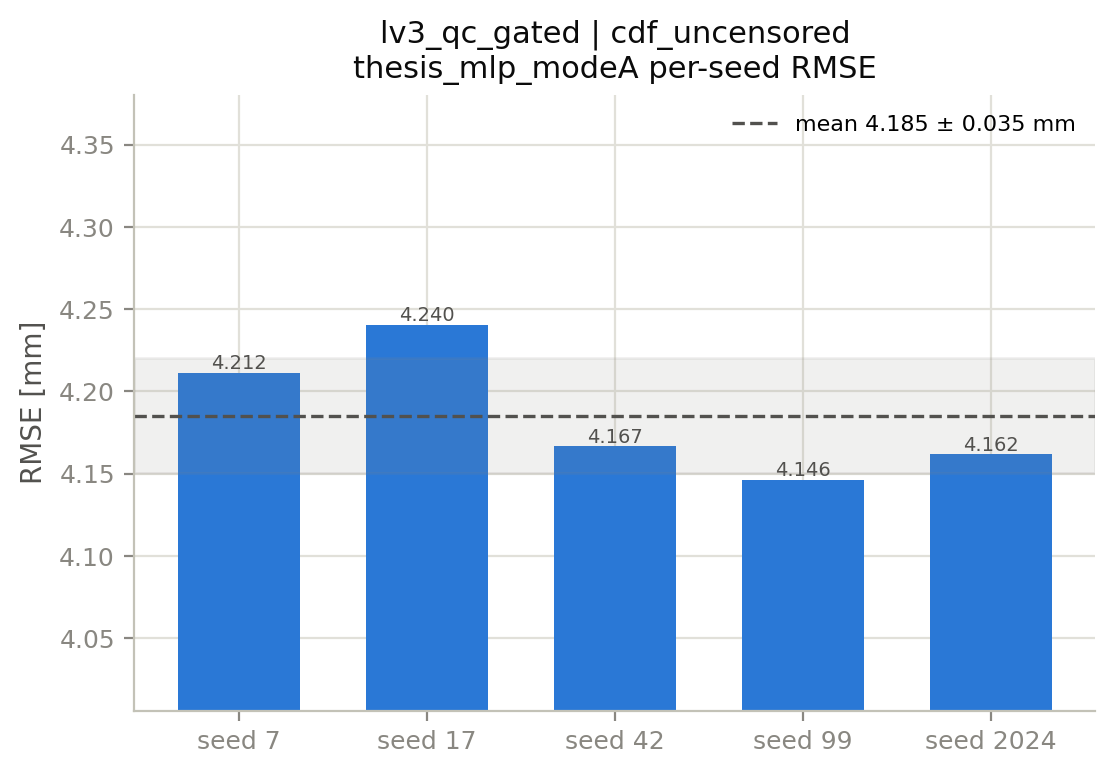
\includegraphics[width=0.80\linewidth]{images/eval_20260709/per_seed_rmse_thesis_mlp_modeA.png}
\caption{Per-seed RMSE of the five production training repetitions (seeds 7/17/42/99/2024) on the refreshed QC-gated uncensored CDF table.}
\label{fig:app-per-seed-rmse}
\end{figure}

\begin{figure}[t]
\centering
\begin{minipage}{0.49\linewidth}
\centering
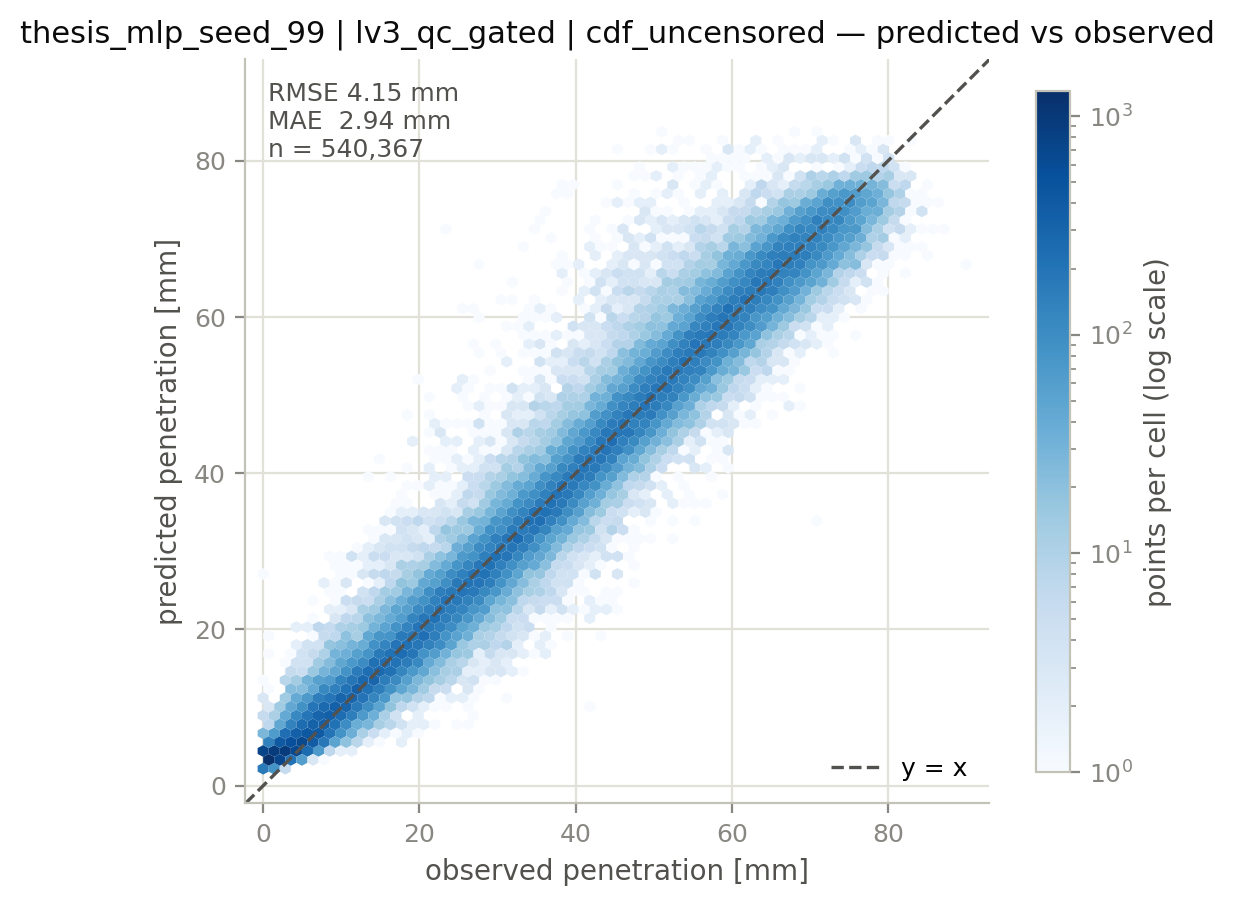
\includegraphics[width=\linewidth]{images/eval_20260709/mlp_seed99_pred_vs_actual.png}
\end{minipage}
\hfill
\begin{minipage}{0.49\linewidth}
\centering
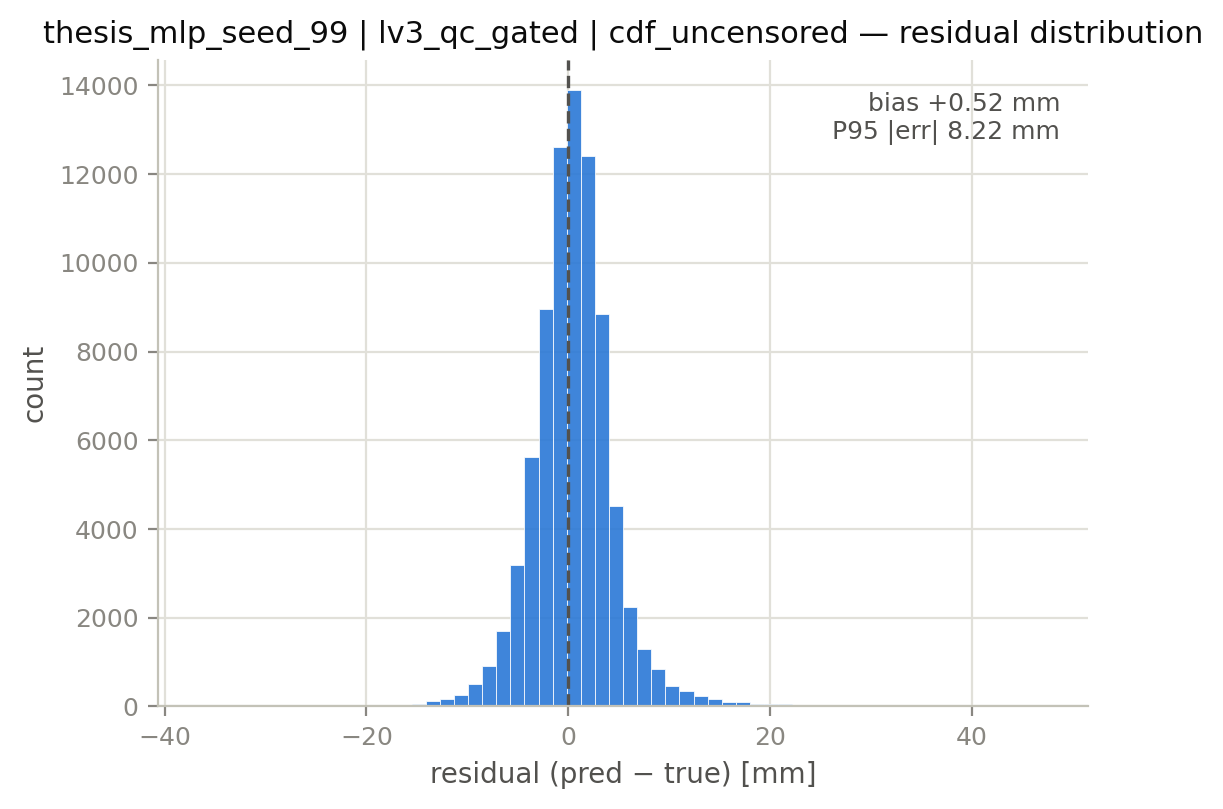
\includegraphics[width=\linewidth]{images/eval_20260709/mlp_seed99_residual_histogram.png}
\end{minipage}
\caption{Predicted-versus-measured scatter (left) and residual histogram (right) for the representative seed-99 repetition on the refreshed QC-gated uncensored CDF table.}
\label{fig:app-seed99-diagnostics}
\end{figure}

\begin{figure}[p]
\centering
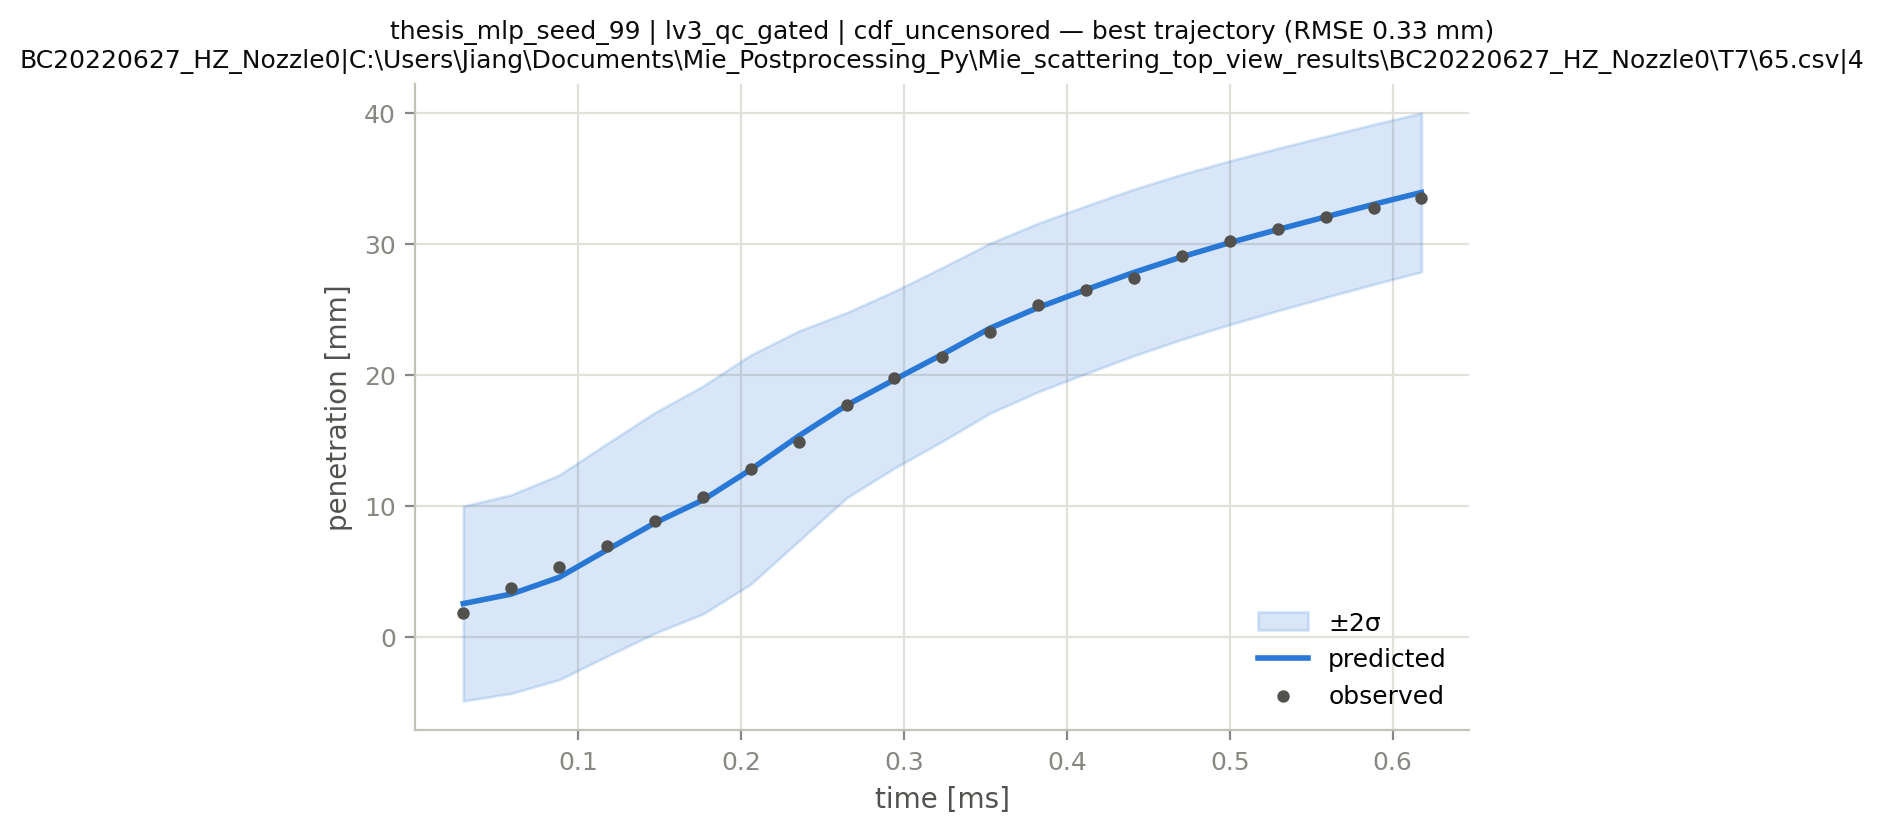
\includegraphics[width=0.94\linewidth]{images/eval_20260709/mlp_seed99_trajectory_best.png}\\[0.8em]
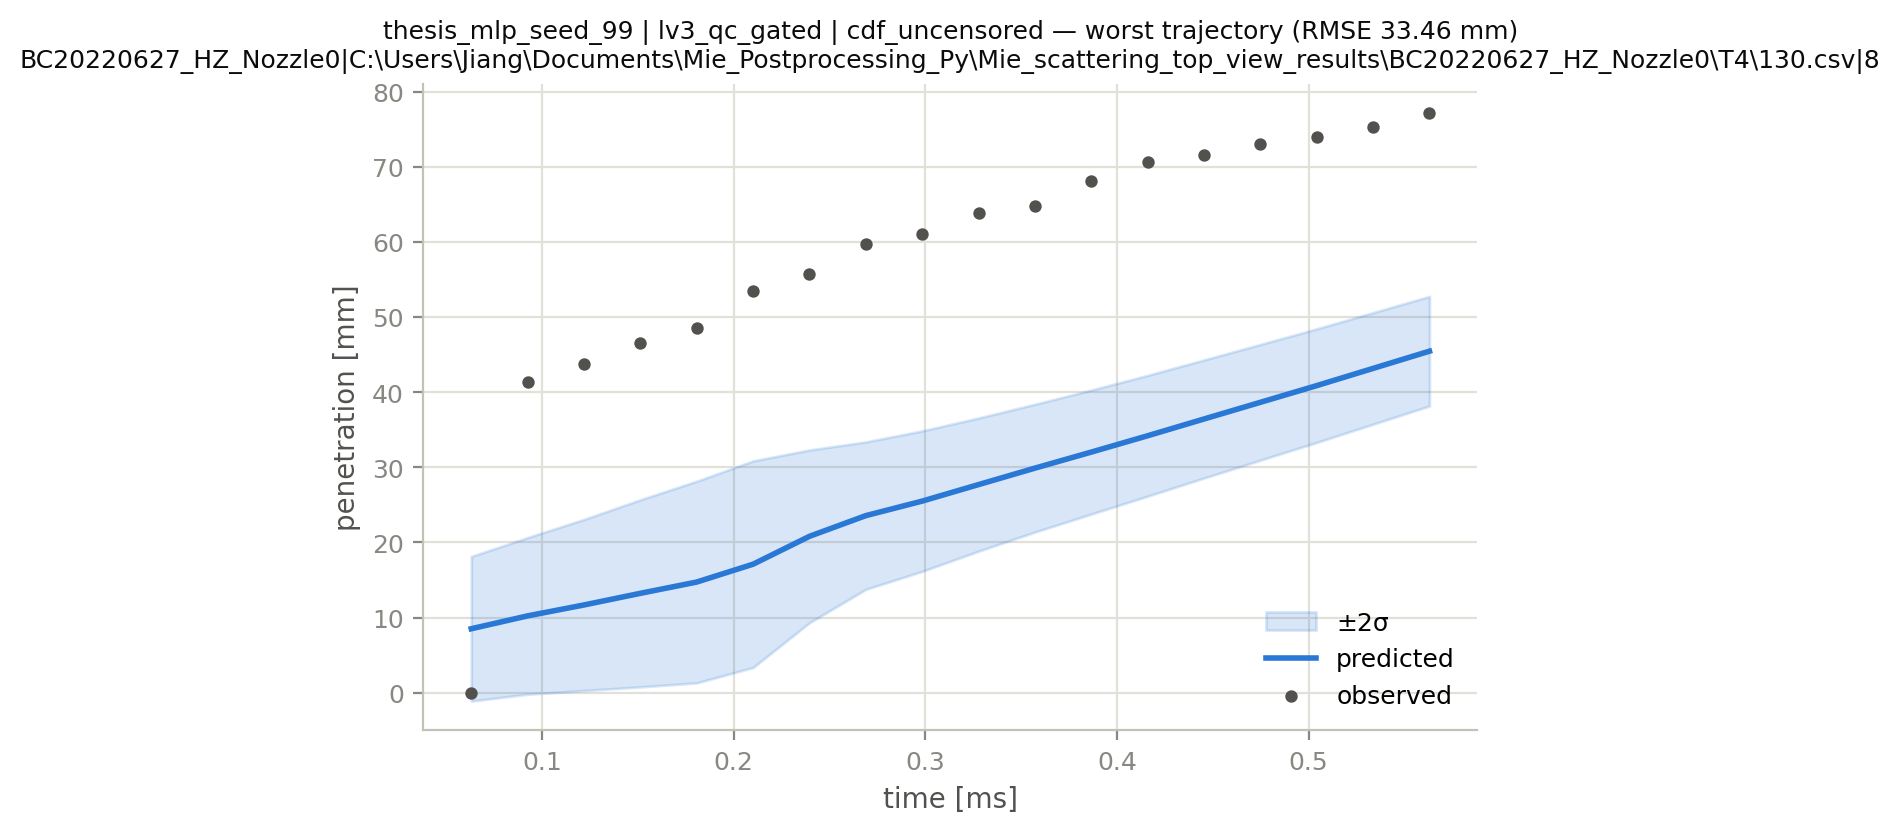
\includegraphics[width=0.94\linewidth]{images/eval_20260709/mlp_seed99_trajectory_worst.png}
\caption{Automatically selected best-fit (top) and worst-fit (bottom) held-out trajectories for the seed-99 repetition on the refreshed table; the selection criterion is the lowest and highest single-trajectory RMSE. The worst case reproduces the transient shape mismatch discussed in the Nozzle-3 failure-mode check of Chapter~5.}
\label{fig:app-seed99-trajectories}
\end{figure}

\begin{figure}[t]
\centering
\begin{minipage}{0.49\linewidth}
\centering
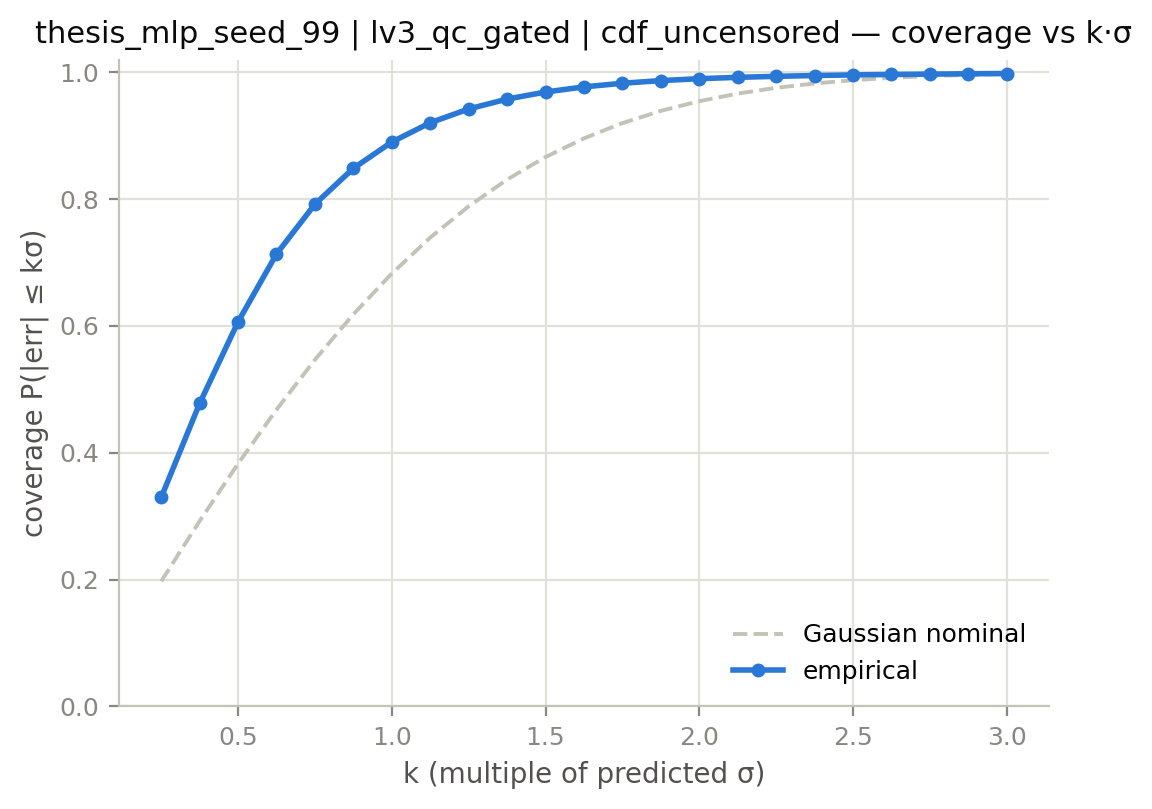
\includegraphics[width=\linewidth]{images/eval_20260709/mlp_seed99_coverage_curve.png}
\end{minipage}
\hfill
\begin{minipage}{0.49\linewidth}
\centering
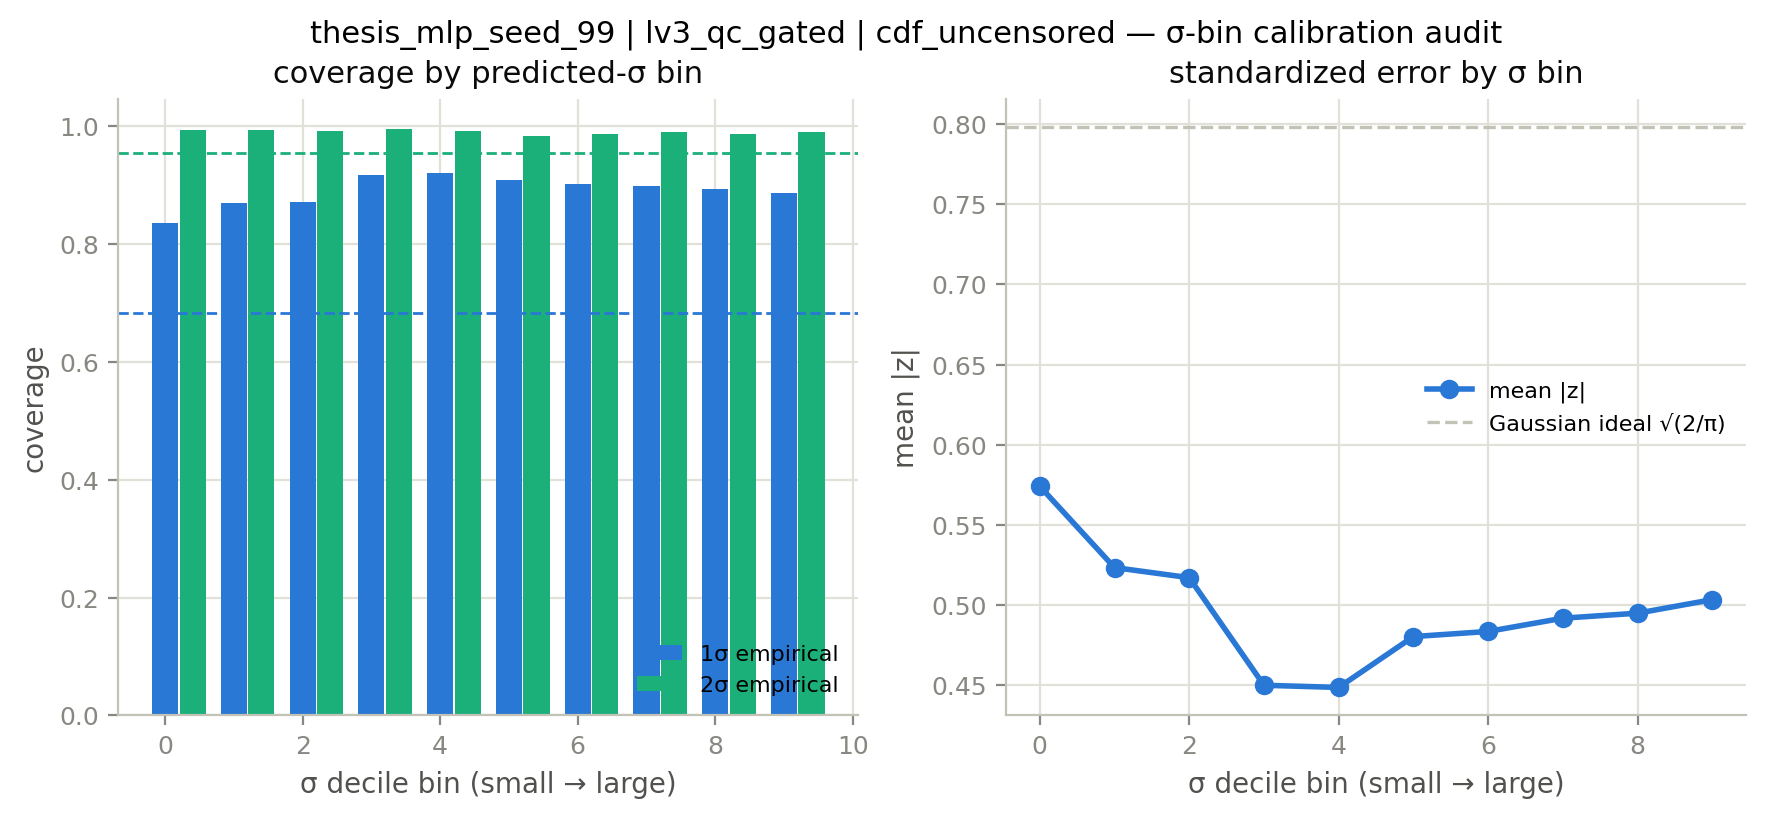
\includegraphics[width=\linewidth]{images/eval_20260709/mlp_seed99_sigma_bin_calibration.png}
\end{minipage}
\caption{Refreshed uncertainty audit for the seed-99 repetition: empirical coverage curve (left) and calibration binned by predicted $\sigma$ (right). These replace the archived calibration coverage audit of the pre-restructure chapter.}
\label{fig:app-seed99-calibration}
\end{figure}

\begin{figure}[t]
\centering
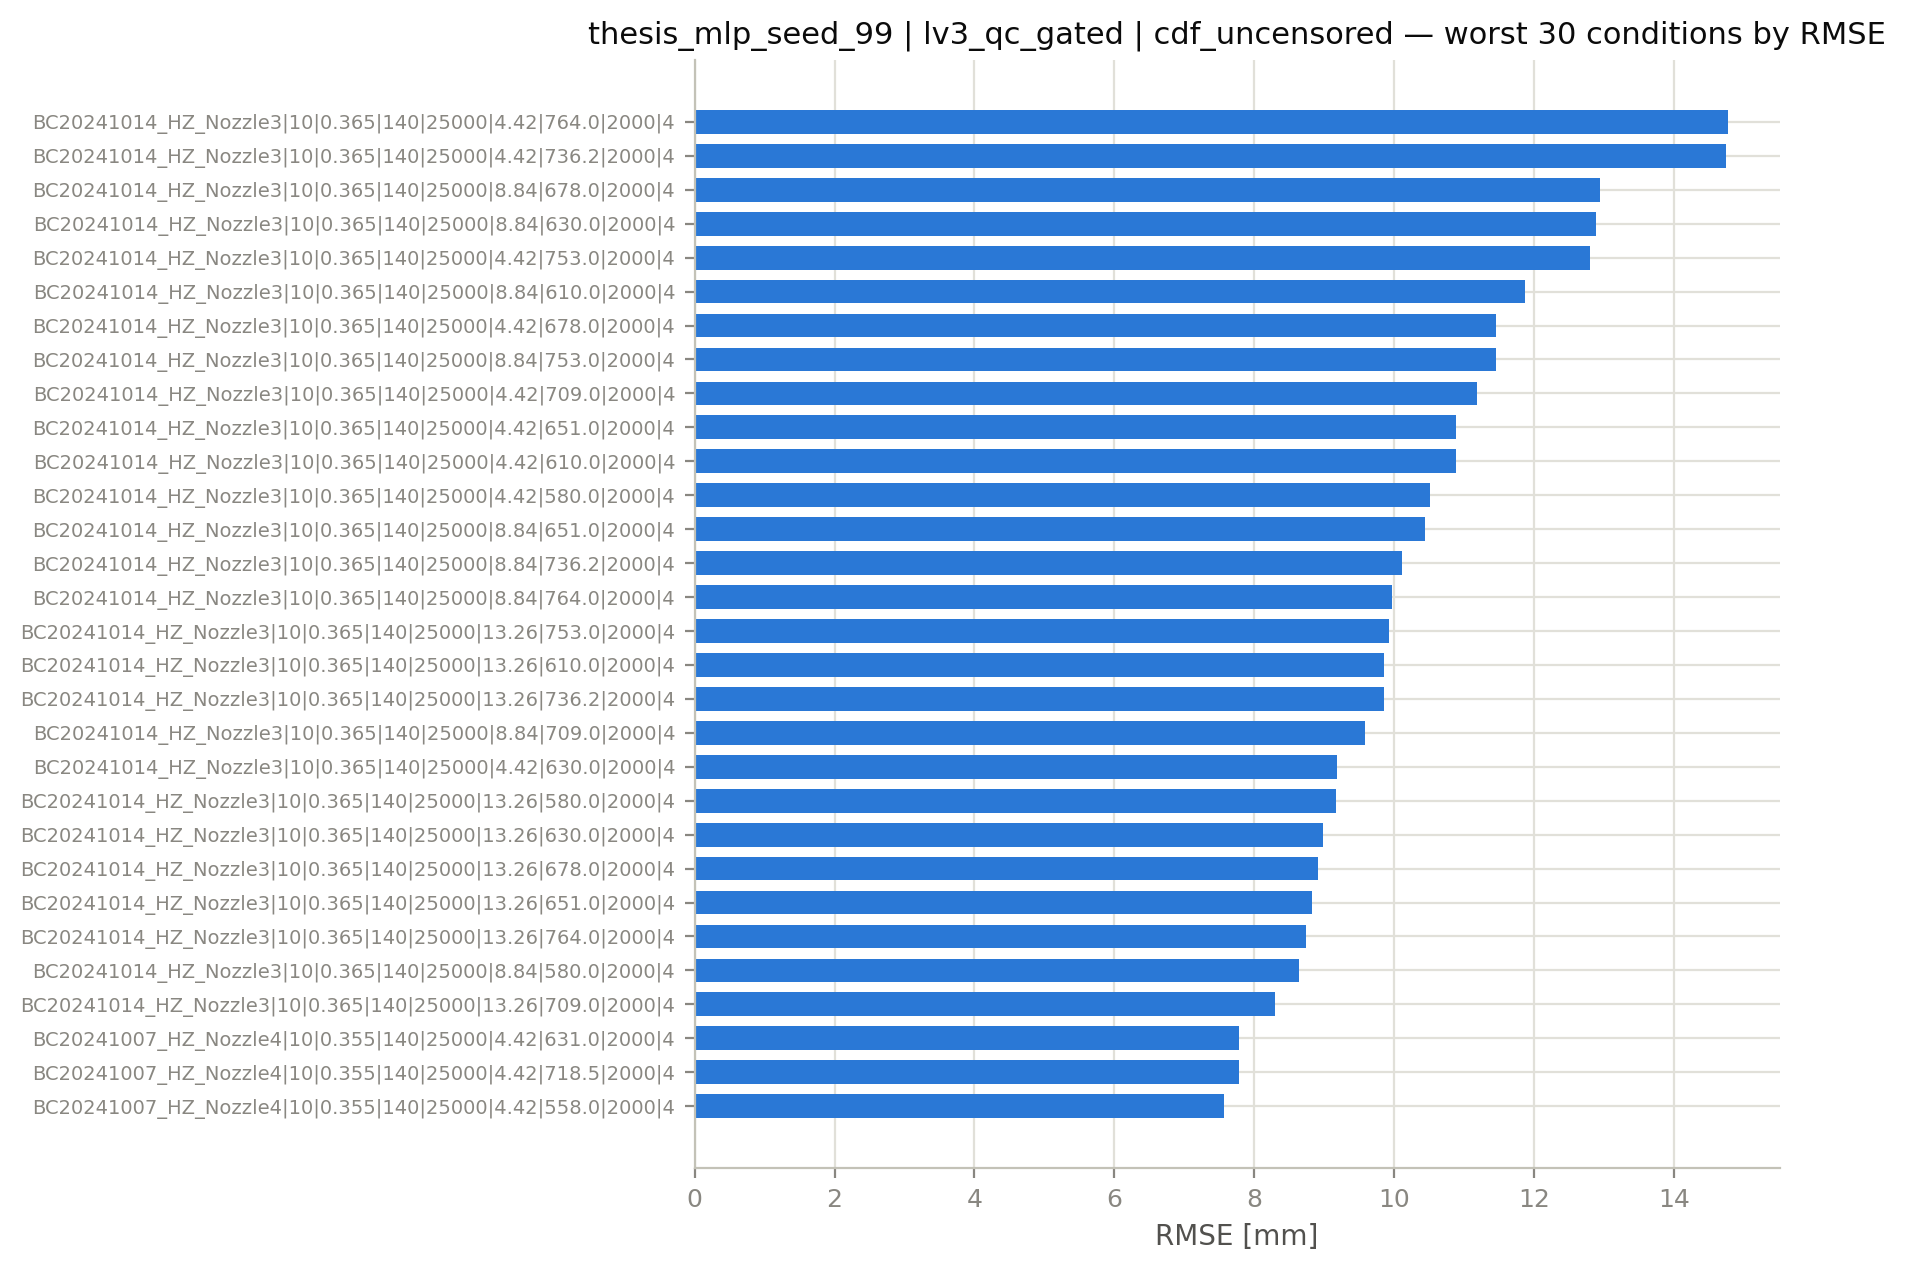
\includegraphics[width=0.88\linewidth]{images/eval_20260709/mlp_seed99_per_condition_rmse.png}
\caption{Per-condition RMSE for the seed-99 repetition on the refreshed QC-gated uncensored CDF table, replacing the archived per-folder RMSE diagnostic. Errors remain unevenly distributed across conditions, consistent with the campaign-folder spread reported in the pre-restructure chapter (easiest folders in the low \SI{3}{mm} range, hardest near \SI{9}{mm}).}
\label{fig:app-per-condition-rmse}
\end{figure}

\FloatBarrier

\subsection{Curriculum-Ablation Detail (Archived LONO)}

The tables below preserve the full archived LONO ablation evidence condensed in
Chapter~5: the Stage-2 anchor-schedule comparison with bias and coverage
columns, its per-fold breakdown, and the four-variant Stage-3 supervision-mix
ranking. All values are archived single-seed (42) five-fold LONO results; the
$\pm$ terms are cross-fold standard deviations.

\begin{table}[t]
\centering
\footnotesize
\setlength{\tabcolsep}{4pt}
\begin{tabular}{@{}L{0.30\linewidth}rrrr@{}}
\toprule
Variant & RMSE [mm] & MAE [mm] & Bias [mm] & 1$\sigma$ / 2$\sigma$ Coverage \\
\midrule
\texttt{no\_anchor}        & 14.54 $\pm$ 12.36 & 10.80 $\pm$ \phantom{0}9.96 & $-8.50 \pm 11.03$ & 0.602 / 0.763 \\
\texttt{mu\_anchor}        & \textbf{12.73 $\pm$ 12.44} & \textbf{\phantom{0}9.86 $\pm$ 10.22} & \textbf{\boldmath$-7.11 \pm 11.51$} & 0.570 / \textbf{0.775} \\
\texttt{mu\_sigma\_anchor} & 13.05 $\pm$ 12.46 & 10.06 $\pm$ 10.33 & $-7.59 \pm 11.45$ & 0.564 / 0.764 \\
\bottomrule
\end{tabular}
\caption{Stage~2 anchor schedule LONO ablation (archived). Each row reports the held-out mean~$\pm$~standard deviation across 5 leave-one-nozzle-out folds (Nozzle0, Nozzle1, Nozzle2, Nozzle4, Nozzle5). The selected Stage~2 teacher configuration is the $\mu$-anchor-only variant, which simultaneously wins in RMSE, MAE, bias magnitude, and 2$\sigma$ coverage.}
\label{tab:stage2-anchor-ablation}
\end{table}

\begin{table}[t]
\centering
\footnotesize
\setlength{\tabcolsep}{4pt}
\begin{tabular}{@{}L{0.28\linewidth}rrrrr|r@{}}
\toprule
Variant & Nozzle0 & Nozzle1 & Nozzle2 & Nozzle4 & Nozzle5 & Mean \\
\midrule
\texttt{no\_anchor}        & 34.25 & \phantom{0}6.56 & 19.18 & 7.57 & 5.11 & 14.54 \\
\texttt{mu\_anchor}        & 34.92 & \phantom{0}7.16 & \textbf{\phantom{0}7.76} & 8.20 & 5.60 & \textbf{12.73} \\
\texttt{mu\_sigma\_anchor} & 35.12 & \phantom{0}7.10 & 10.04 & 7.73 & 5.27 & 13.05 \\
\bottomrule
\end{tabular}
\caption{Per-fold LONO RMSE [mm] for the three Stage~2 anchor variants (archived). All three fail on the Nozzle0 fold (the factory-fresh reference nozzle, a true cross-design-family extrapolation, dominant by point count). The differentiating fold is Nozzle2, where omitting the anchor increases RMSE by \SI{11.4}{mm} compared to the $\mu$-anchor-only variant.}
\label{tab:stage2-anchor-ablation-per-fold}
\end{table}

\begin{table}[t]
\centering
\footnotesize
\begin{tabular}{lrrrrr}
\toprule
Configuration & RMSE [mm] & MAE [mm] & Bias [mm] & 1$\sigma$ Coverage & 2$\sigma$ Coverage \\
\midrule
Baseline configuration & 12.68 $\pm$ 12.74 & 9.97 $\pm$ 10.55 & $-7.86 \pm 11.28$ & 0.565 & 0.759 \\
Reliable-regime-only pure raw variant & 12.76 $\pm$ 12.48 & 10.01 $\pm$ 10.22 & $-7.45 \pm 11.35$ & 0.556 & 0.761 \\
\textbf{Uncertain-regime mixed variant} & \textbf{12.55 $\pm$ 12.46} & \textbf{9.80 $\pm$ 10.18} & \textbf{\boldmath$-6.87 \pm 11.53$} & \textbf{0.575} & 0.770 \\
Anchor-off variant & 12.73 $\pm$ 12.44 & 9.86 $\pm$ 10.22 & $-7.11 \pm 11.51$ & 0.570 & \textbf{0.775} \\
\bottomrule
\end{tabular}
\caption{Stage~3 LONO ablation after fixing the Stage~2 teacher to $\mu$-anchor-only (archived). Each row reports the held-out mean~$\pm$~standard deviation across five leave-one-nozzle-out folds. The uncertain-regime mixed variant wins in RMSE/MAE; the anchor-off variant exhibits the strongest 2$\sigma$ coverage. Nozzle0 remains a cross-design-family failure for every variant (RMSE \SIrange{34.76}{35.31}{mm}, bias $\approx\SI{-27}{mm}$).}
\label{tab:stage3-ablation-ranking}
\end{table}

\begin{figure}[t]
\centering
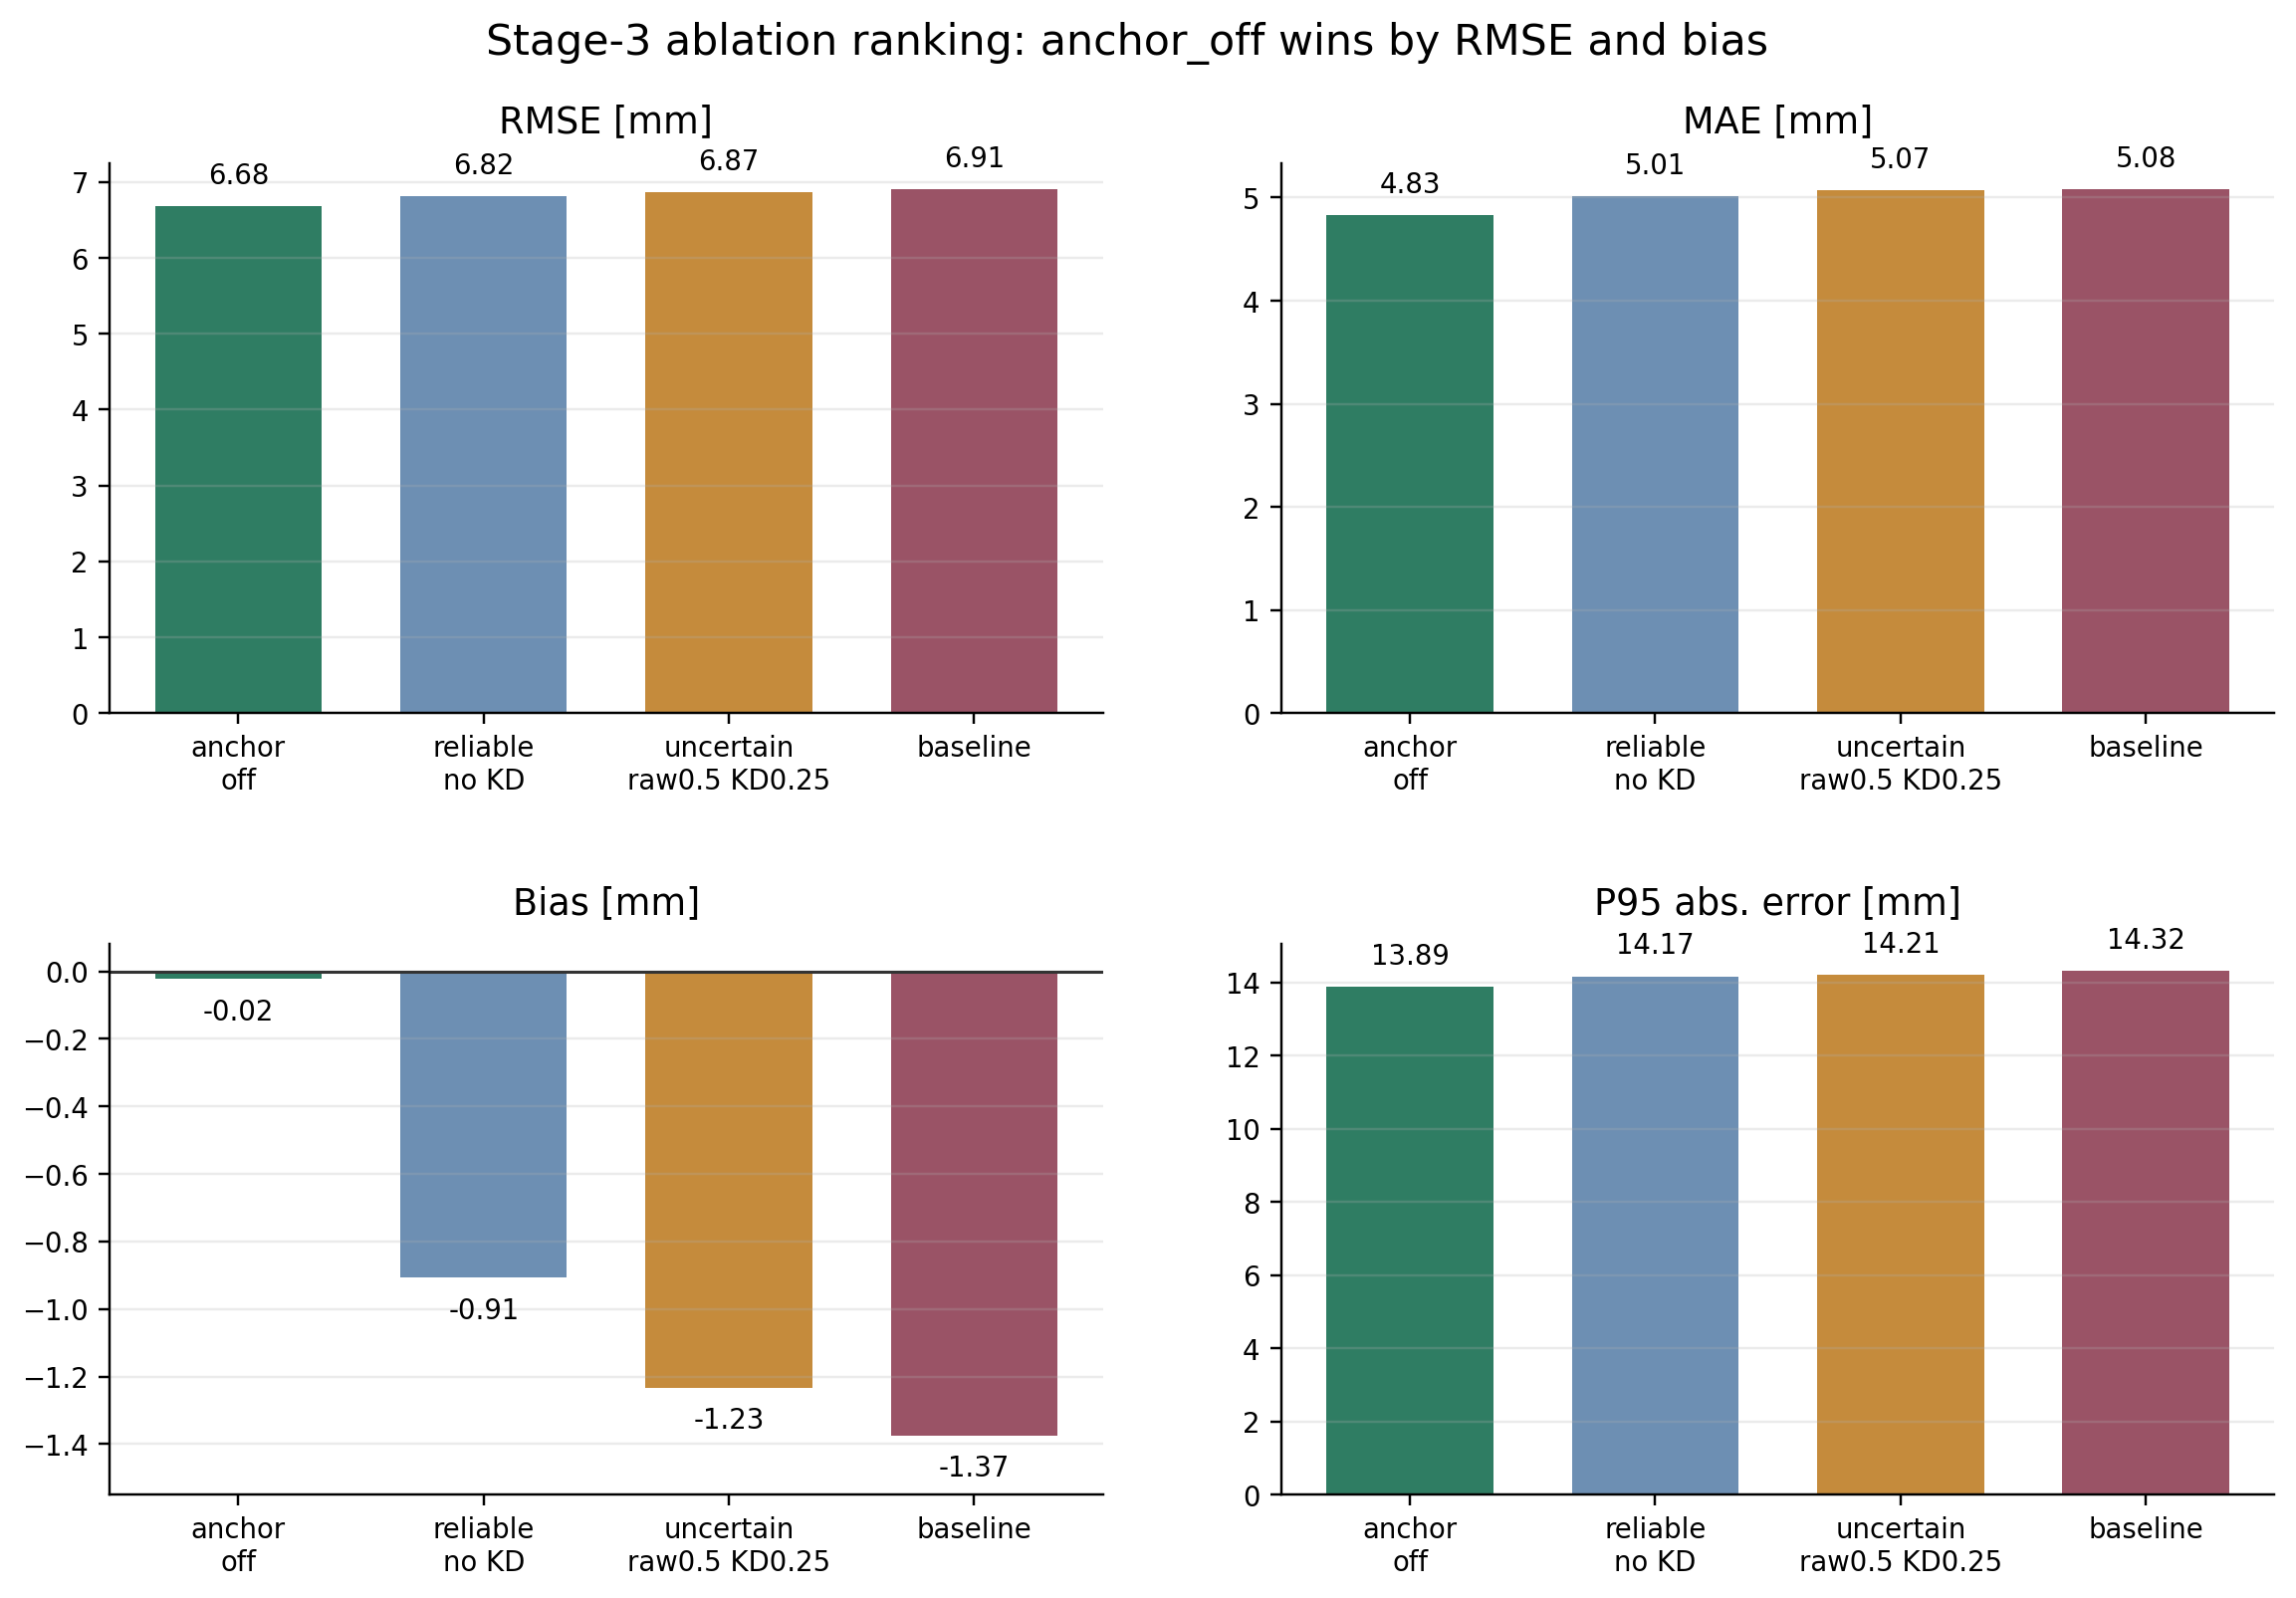
\includegraphics[width=\linewidth]{images/neural_network_fit_results/ablation_comparison_best.png}
\caption{Summary of the archived Stage~3 LONO tuning. After fixing the Stage~2 teacher to $\mu$-anchor-only, the uncertain-regime mixed variant obtained the lowest average RMSE/MAE, while the anchor-off variant provided the strongest 2$\sigma$ coverage. Source artifact paths are found in Appendix~\ref{app:implementation_mapping}.}
\label{fig:ablation-best}
\end{figure}

\FloatBarrier

\subsection{KD-Form Study: Supervision-Regime and Censoring Slices (Archived)}

Chapter~5 reports the mechanism and the headline outcome of the distillation
loss fix. The archived slice-level evidence is preserved here. The mixed
distillation loss combines a mean MSE with a log-variance MSE,
\begin{equation}
\mathcal{L}_{\mathrm{KD}} \;=\; (\mu_s-\mu_t)^{2} \;+\; \lambda_\sigma\,\bigl(\log\sigma_s^{2} - \log\sigma_t^{2}\bigr)^{2},
\label{eq:kd-mse-mu-plus-sigma}
\end{equation}
which re-supervises $\sigma$ explicitly while removing the variance-inflation
escape route permitted by the forward-KL formulation.
Table~\ref{tab:stage3-kd-regimes} breaks the held-out metrics down by training
supervision regime and FOV censoring flag for a single representative seed
(99); the slices were computed on the archived censoring-inclusive set
(692{,}942 points), so its Full Set row is a regime-slice diagnostic rather
than the refreshed headline.

\begin{table}[t]
\centering
\small
\begin{tabular}{lrrrr}
\toprule
Slice & n & RMSE [mm] & Bias [mm] & Median \(|\sigma_s-\sigma_t|\) [mm] \\
\midrule
Full Set & 692{,}942 & 4.76 & +0.72 & 0.82 \\
Reliable Raw Regime & 549{,}299 & 4.68 & +0.67 & 1.00 \\
Uncertain Raw Regime & 64{,}487 & 5.88 & +1.27 & 0.40 \\
Teacher-Only Regime & 79{,}156 & 4.33 & +0.65 & \textbf{0.27} \\
KD-Only (Combined) & 143{,}643 & 5.08 & +0.93 & 0.32 \\
Near Cap (\(\mathrm{pen}\ge 0.9\,\mathrm{cap}\)) & 54{,}704 & 4.89 & \(-\)0.66 & 0.27 \\
Trajectory Uncensored & 393{,}912 & 4.85 & +0.99 & 0.81 \\
Trajectory Censored & 299{,}030 & 4.65 & +0.37 & 0.84 \\
Trajectory Censored \& Near Cap & 47{,}676 & 4.95 & \(-\)0.69 & 0.28 \\
\bottomrule
\end{tabular}
\caption{Archived held-out metrics across slices for the mixed-distillation model (\(\lambda_\sigma=5.0\), seed 99, archived censoring-inclusive set). ``Reliable Raw Regime'' indicates the supervision zone dominated by raw NLL; ``KD-Only'' combines the uncertain raw regime and the teacher-only regime, both fully supervised via Eq.~\eqref{eq:kd-mse-mu-plus-sigma}. The median \(|\sigma_s-\sigma_t|\) compares against the Stage~2 teacher's \(\sigma\) point-by-point to quantify the extent of calibration drift.}
\label{tab:stage3-kd-regimes}
\end{table}

\begin{figure}[t]
\centering
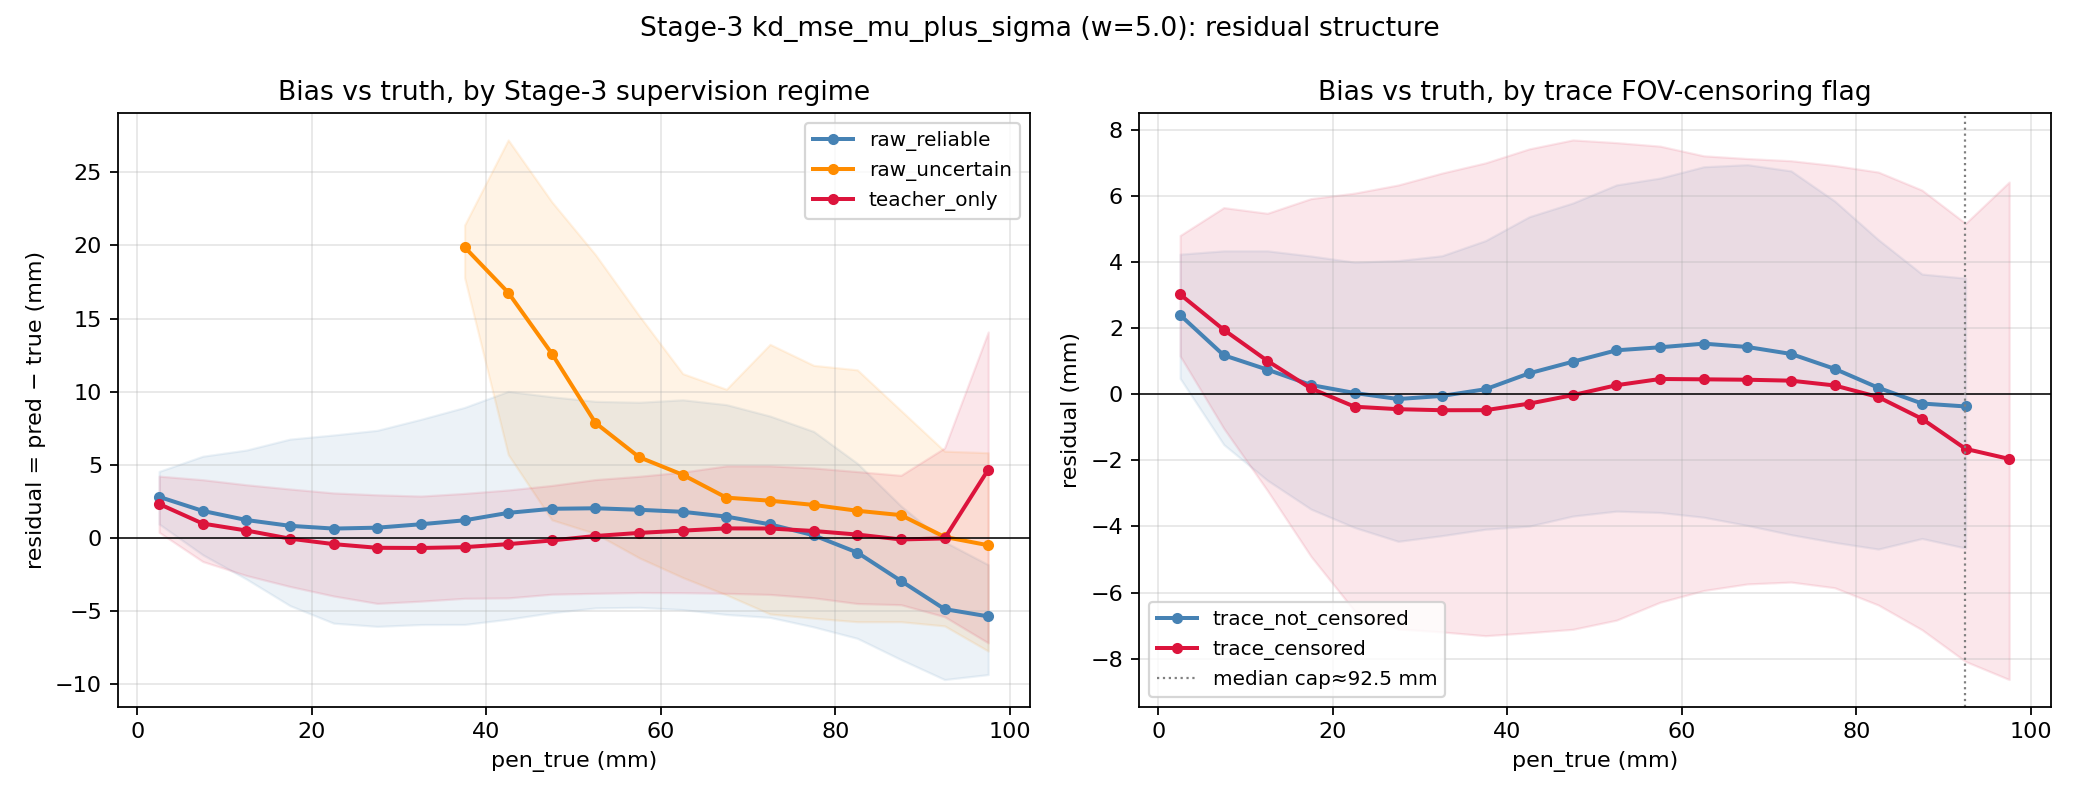
\includegraphics[width=\linewidth]{images/neural_network_fit_results/stage3_kd_mse_mu_plus_sigma_residual_vs_truth.png}
\caption{Archived residual structure for the mixed-distillation model (\(\lambda_\sigma=5\)). Left: categorized by training regime (Reliable Raw / Uncertain Raw / Teacher-Only). Right: categorized by trajectory-level FOV censoring flag. Shaded regions correspond to the P10--P90 residual ranges.}
\label{fig:kd-residual-by-regime}
\end{figure}

\begin{figure}[t]
\centering
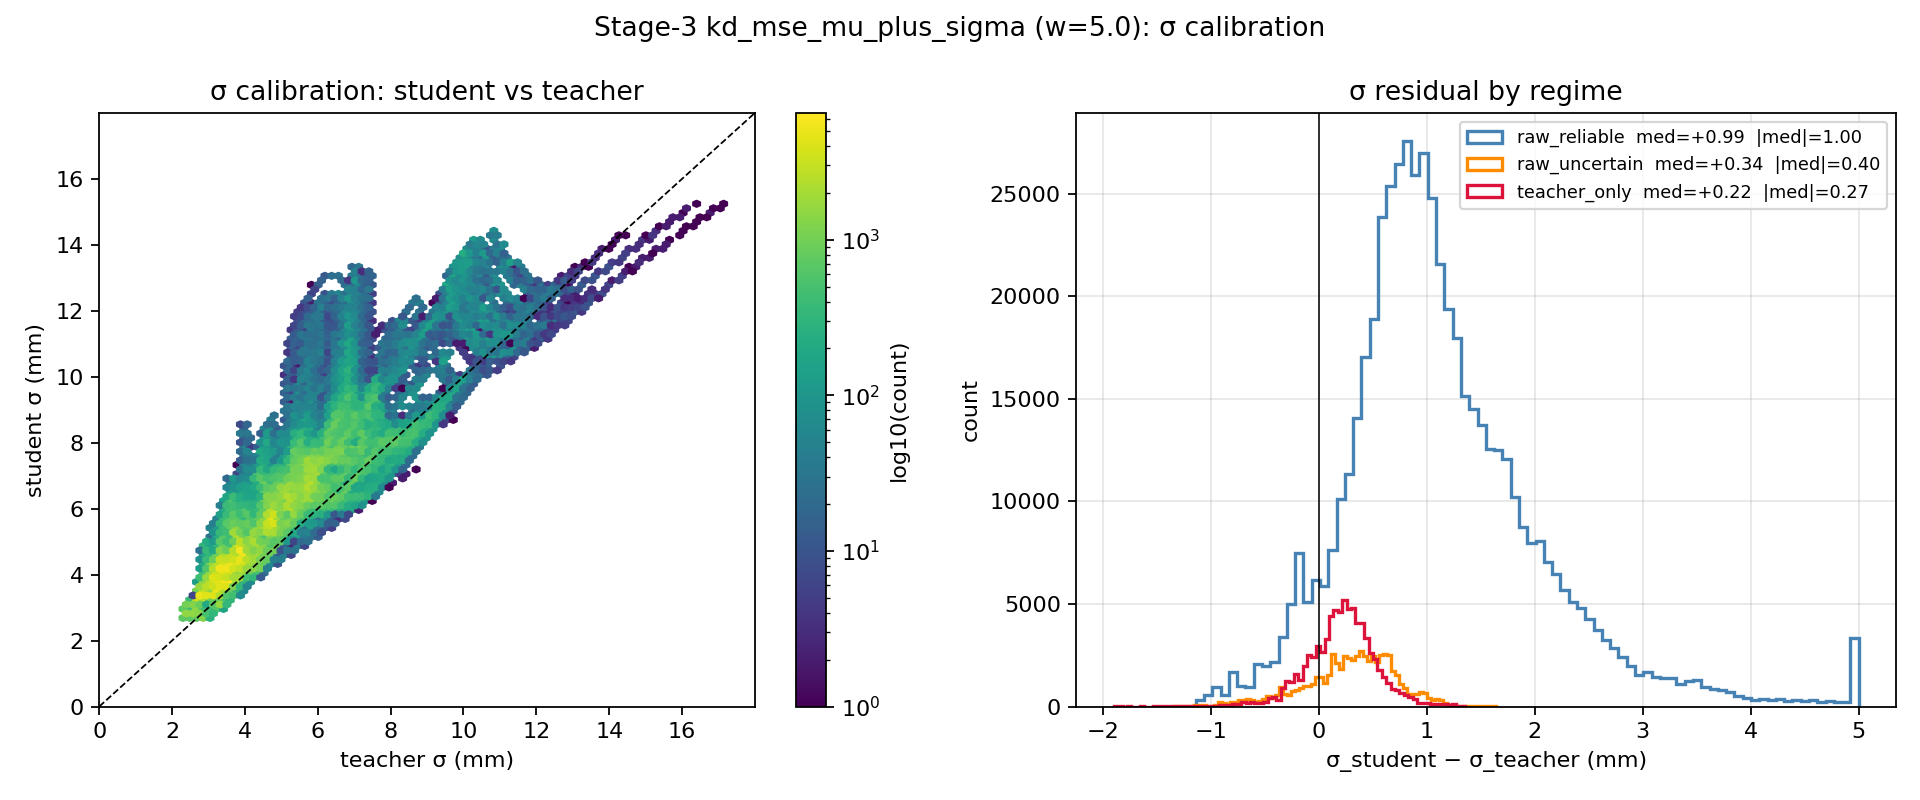
\includegraphics[width=\linewidth]{images/neural_network_fit_results/stage3_kd_mse_mu_plus_sigma_sigma_calibration.png}
\caption{Archived uncertainty calibration profile for the mixed-distillation model (\(\lambda_\sigma=5\)). Left: point-wise hex-bin joint distribution of the student's \(\sigma\) versus the teacher's \(\sigma\). Right: distribution histograms of the residual \(\sigma_s-\sigma_t\) across supervision regimes.}
\label{fig:kd-sigma-calibration}
\end{figure}

\FloatBarrier

\subsection{Residual-Adaptation Detail}

The two tables below are the refreshed detail behind the post-hoc adaptation
summary of Chapter~5: the injector-conditioning design comparison and the full
residual climb with calibration columns. Both are regenerated on the QC-gated
uncensored CDF protocol; they supersede the Level-2-era versions of the
original study. The figures that follow are archived from the 2026-06-08
adaptation study: their annotated values reflect the Level-2-era protocol of
that study, so the refreshed equivalents in the tables take precedence where
they differ.

% --- Refreshed tables (source: 05_results_update_temp/appendix_fragments_residual.tex, verified against metrics_wide.csv of run 20260709_223144) ---
\begin{table}[tbp]
\centering
\footnotesize
\setlength{\tabcolsep}{4pt}
\begin{tabular}{@{}L{0.32\linewidth}rrL{0.28\linewidth}@{}}
\toprule
Injector-conditioning design & RMSE [mm] & 95\% CI [mm] & Fallback for unseen nozzle \\
\midrule
One-hot nozzle input (deployed; five-seed mean) & 4.185 & --- & none (needs a hard-coded identity) \\
Independent per-nozzle heads (\texttt{family\_head\_baseline}) & 4.901 & [4.845, 4.953] & none (training data fragmented) \\
Residual head, zero-init. $\Delta_f$ (\texttt{residual\_fh}) & 4.519 & [4.463, 4.573] & structural (defaults to shared model) \\
\bottomrule
\end{tabular}
\caption{Injector-conditioning designs on the refreshed QC-gated uncensored CDF protocol (540{,}367 points). Values are from \texttt{evalrun\_\allowbreak{}20260709\_\allowbreak{}223144\_\allowbreak{}thesis\_\allowbreak{}full\_\allowbreak{}fullclean\_\allowbreak{}bootstrap\_\allowbreak{}fast\_\allowbreak{}20260709\_\allowbreak{}223142}; cluster-bootstrap 95\% confidence intervals are shown for the single-checkpoint designs available directly in \texttt{metrics\_wide.csv}, while the deployed result is the five-seed production-MLP mean.}
\label{tab:residual-family-designs}
\end{table}

\begin{table}[tbp]
\centering
\footnotesize
\setlength{\tabcolsep}{3.5pt}
\begin{tabular}{@{}L{0.31\linewidth}rrrrrr@{}}
\toprule
Model & RMSE & MAE & ECE & CRPS & P50 & QC-retrained RMSE \\
\midrule
Naber--Siebers (reference) & 9.212 & 7.154 & --- & 5.109 & 8.983 & --- \\
Production MLP, five-seed mean (reference) & 4.185 & 2.978 & --- & 2.301 & 2.831 & --- \\
Single-output SVGP (reference) & 4.087 & 2.857 & 0.0214 & 2.063 & 2.516 & --- \\
\midrule
\texttt{family\_head\_baseline} & 4.901 & 3.518 & 0.0727 & 2.688 & 3.785 & --- \\
\texttt{residual\_fh} & 4.519 & 3.147 & 0.0612 & 2.351 & 3.264 & 4.590 \\
\texttt{residual\_film} & 4.401 & 3.035 & 0.0413 & 2.212 & 3.035 & 4.400 \\
\texttt{residual\_svgp} & \textbf{3.921} & \textbf{2.800} & \textbf{0.0267} & \textbf{2.019} & \textbf{2.026} & \textbf{3.848} \\
\bottomrule
\end{tabular}
\caption{Refreshed \texttt{lv3\_qc\_gated} residual-model climb from \texttt{evalrun\_\allowbreak{}20260709\_\allowbreak{}223144\_\allowbreak{}thesis\_\allowbreak{}full\_\allowbreak{}fullclean\_\allowbreak{}bootstrap\_\allowbreak{}fast\_\allowbreak{}20260709\_\allowbreak{}223142}. RMSE, MAE, CRPS, P50, and QC-retrained RMSE are in mm; ECE is unitless. CDF metrics use the \texttt{cdf\_uncensored} protocol (540{,}367 points), whereas P50 is RMSE under \texttt{p50\_observed} (4{,}215 points); these values must not be mixed with the earlier 542{,}565-point Level-2 table. The residual-SVGP and QC-retrained residual-SVGP variants were not evaluated under a matched LONO protocol.}
\label{tab:residual-climb}
\end{table}

\begin{figure}[t]
\centering
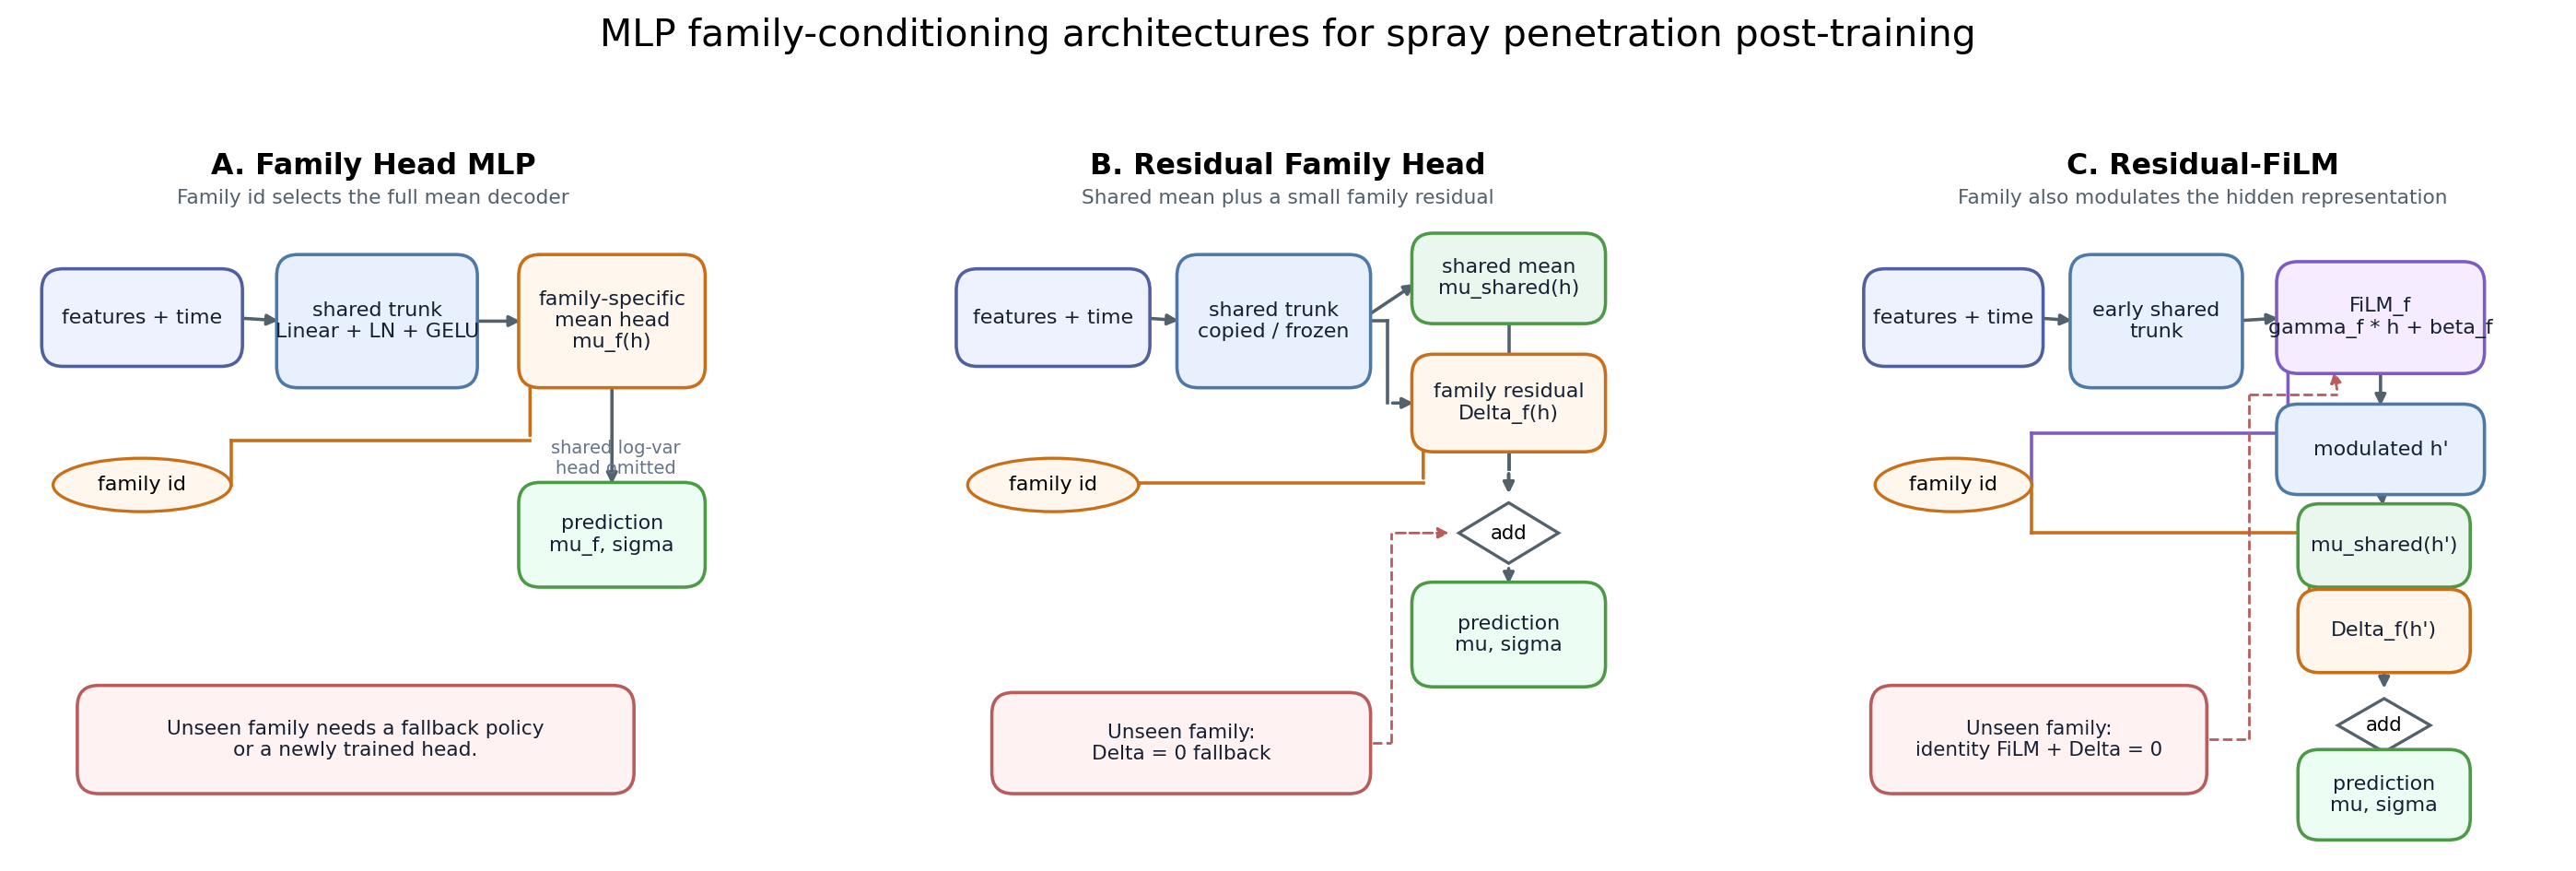
\includegraphics[width=0.96\linewidth]{images/residual_family_head_20260608/mlp_family_conditioning_architecture.png}
\caption{Injector-conditioning designs (archived study): independent per-nozzle head, additive residual head, and FiLM modulation. Grey blocks are frozen (hot-started from the deployed Stage~3 checkpoint); green blocks are the small trainable per-nozzle components.}
\label{fig:residual-architecture}
\end{figure}

\begin{figure}[t]
\centering
\begin{minipage}{0.49\linewidth}
\centering
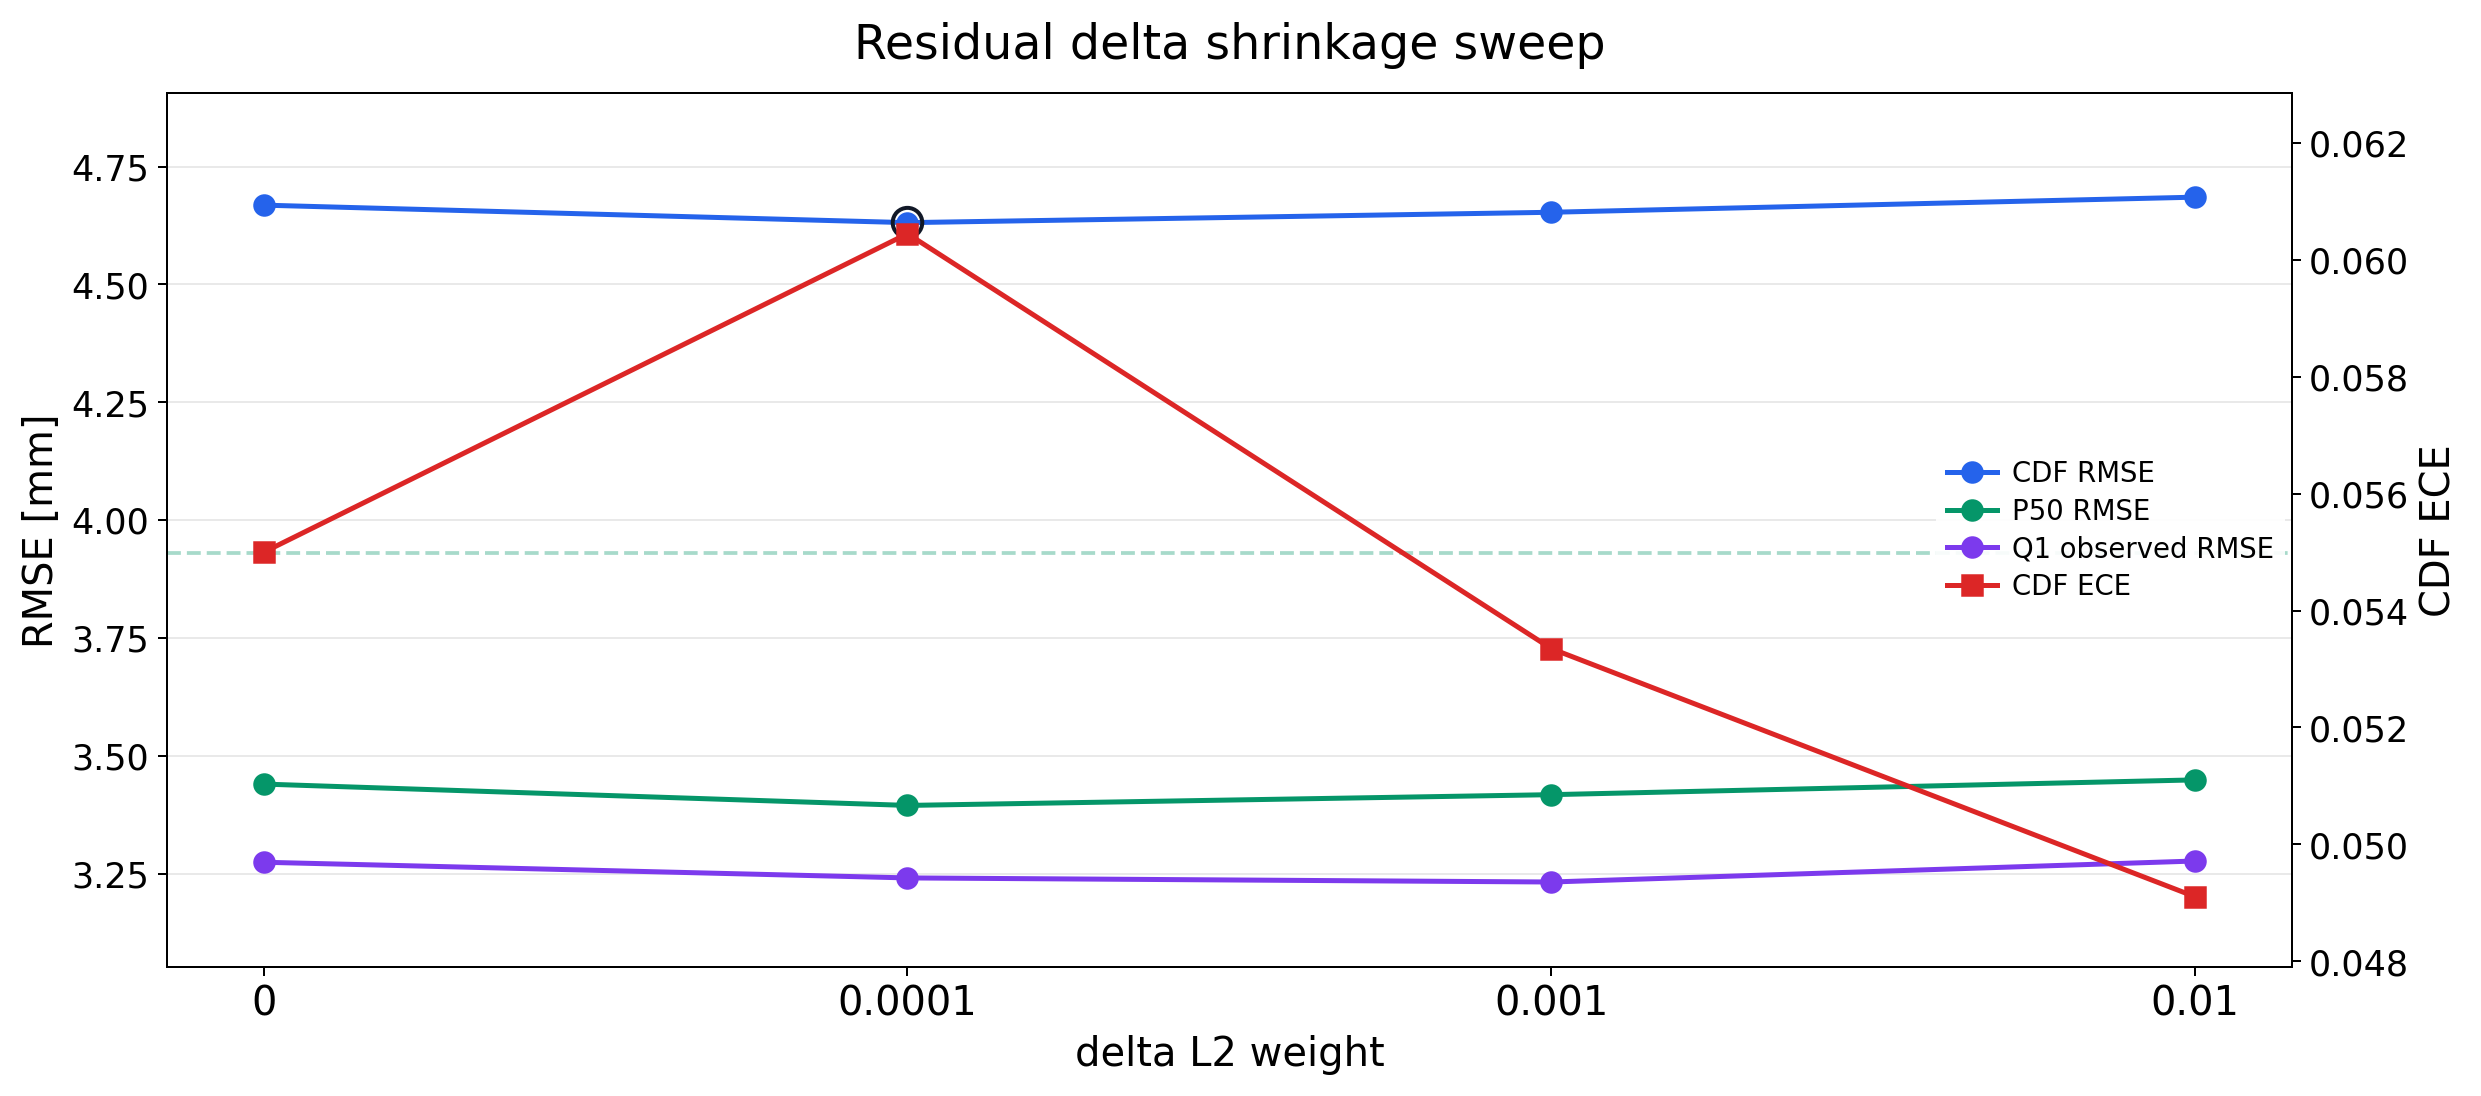
\includegraphics[width=\linewidth]{images/residual_family_head_20260608/delta_l2_sweep.png}
\end{minipage}
\hfill
\begin{minipage}{0.49\linewidth}
\centering
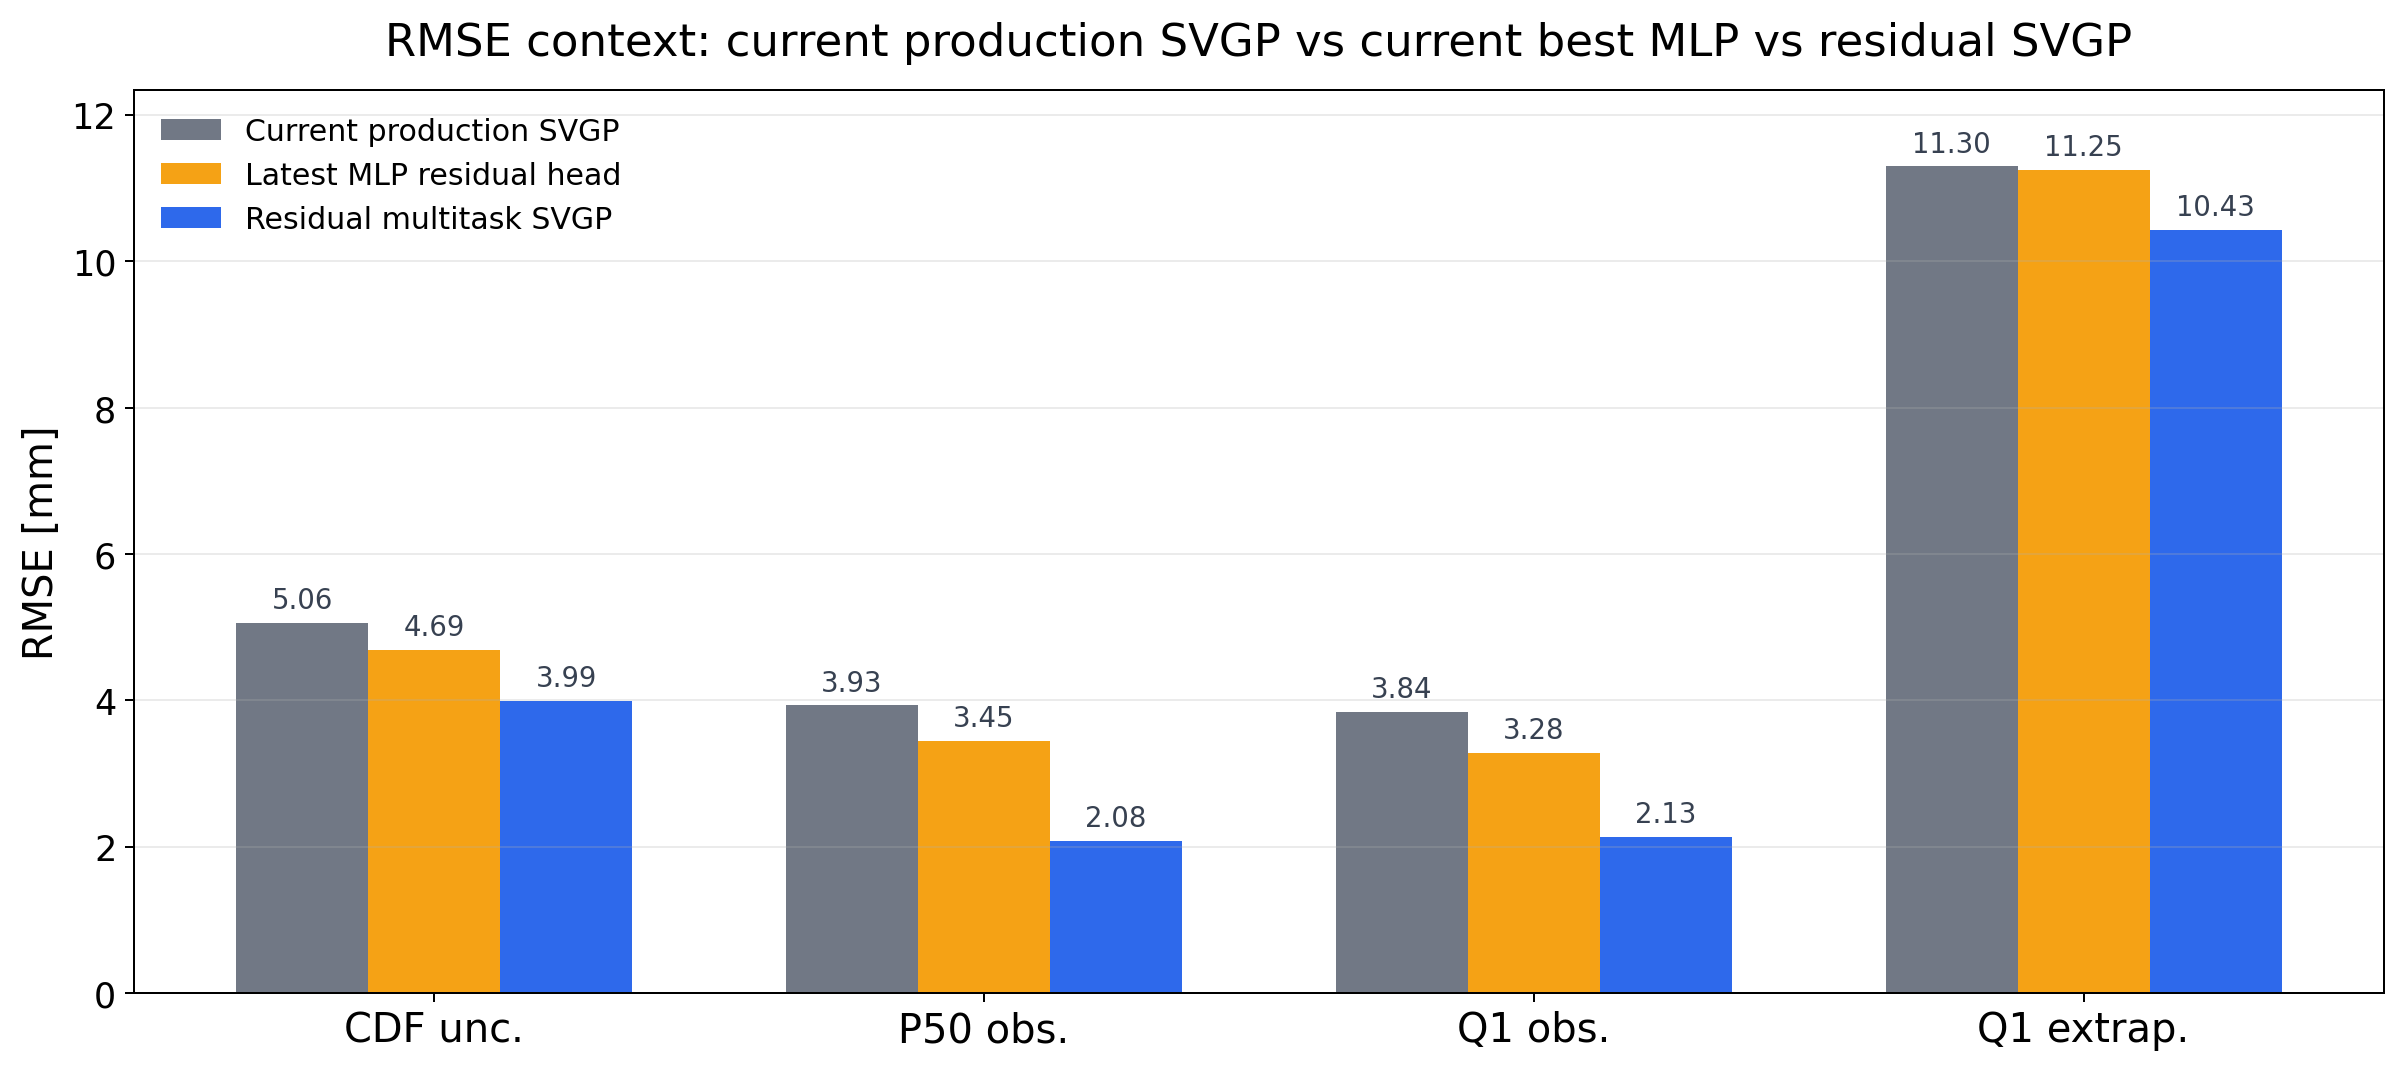
\includegraphics[width=\linewidth]{images/residual_family_head_20260608/residual_svgp_context_rmse_comparison.png}
\end{minipage}
\caption{Archived adaptation-study diagnostics (Level-2-era values). Left: shrinkage sweep for the residual head ($\lambda_\Delta\in\{0,10^{-4},10^{-3},10^{-2}\}$); every setting beats the independent-head fallback. Right: the additive-residual multi-task SVGP against the prior best on the same table. The refreshed QC-gated values are given in Table~\ref{tab:residual-climb}.}
\label{fig:residual-svgp-climb}
\label{fig:residual-delta-sweep}
\end{figure}

\begin{table}[t]
\centering
\footnotesize
\begin{tabular}{@{}L{0.30\linewidth}rrr@{}}
\toprule
Arm & In-family RMSE & All-5 RMSE & In-family bias \\
 & (4 folds, mm) & (5 folds, mm) & (mm) \\
\midrule
Deployed nozzle head & 7.44 $\pm$ 1.46 & 8.32 $\pm$ 2.33 & +5.07 \\
Residual head & \textbf{5.16 $\pm$ 0.65} & 6.95 $\pm$ 4.05 & +0.78 \\
Residual-FiLM & 5.15 $\pm$ 0.67 & 6.96 $\pm$ 4.08 & +0.75 \\
\bottomrule
\end{tabular}
\caption{Archived LONO transfer of the residual conversion on the MLP arms (hold out N1/N2/N4/N5/N6 one at a time, N0 in training, trained from scratch per fold). The in-family aggregate excludes the out-of-design-family N6 stress fold. The residual conversion cuts in-family RMSE by $\approx$31\% and repairs the mean bias; FiLM and the plain residual head are indistinguishable under transfer.}
\label{tab:residual-lono}
\end{table}

\begin{figure}[t]
\centering
\begin{minipage}{0.49\linewidth}
\centering
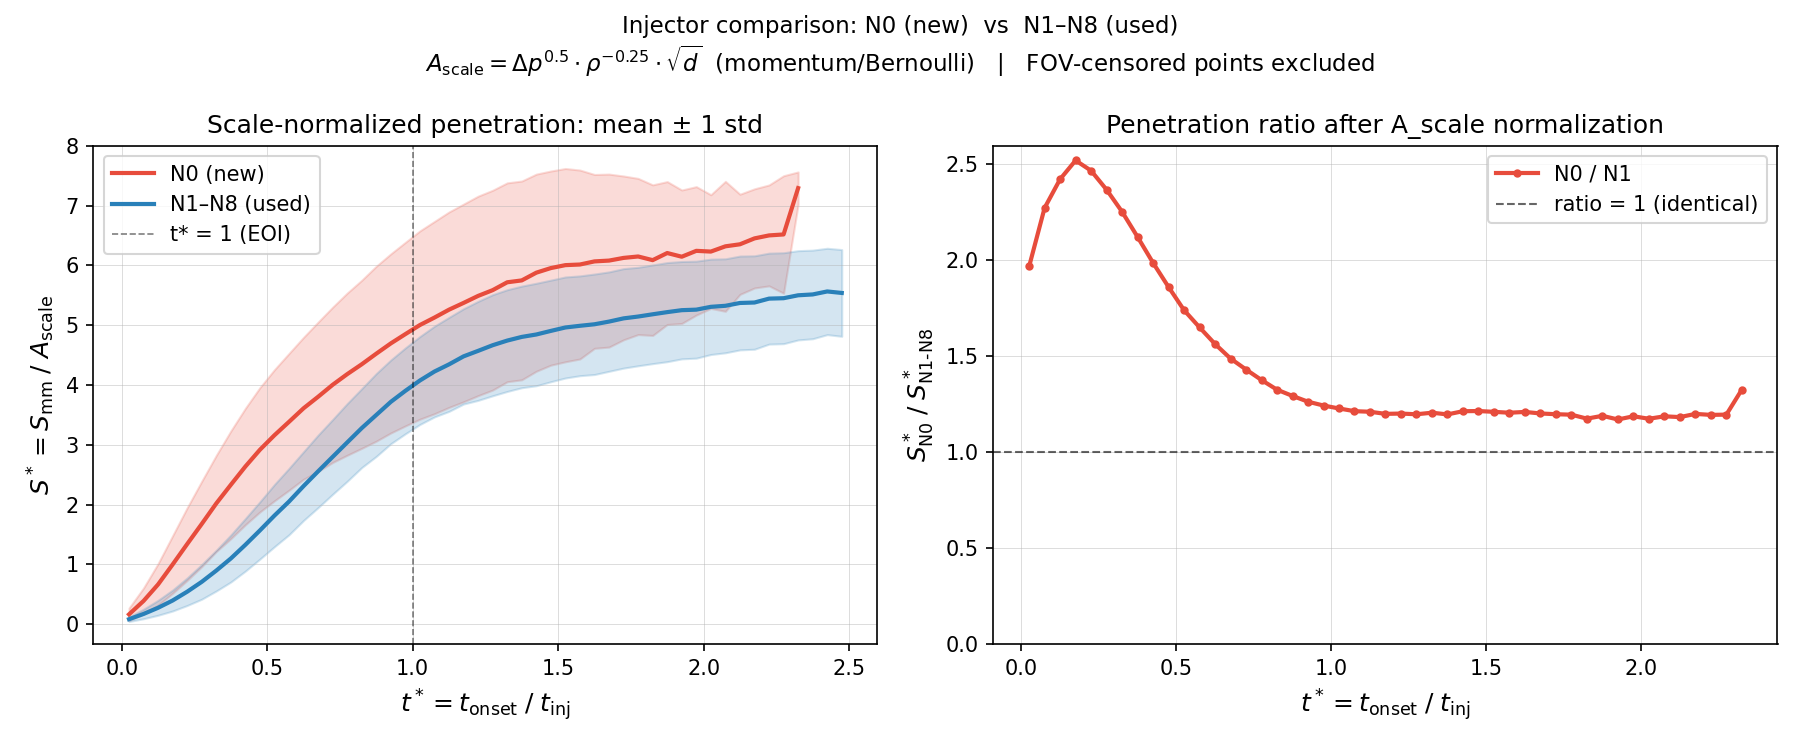
\includegraphics[width=\linewidth]{images/residual_family_head_20260608/injector_comparison_dp050.png}
\end{minipage}
\hfill
\begin{minipage}{0.49\linewidth}
\centering
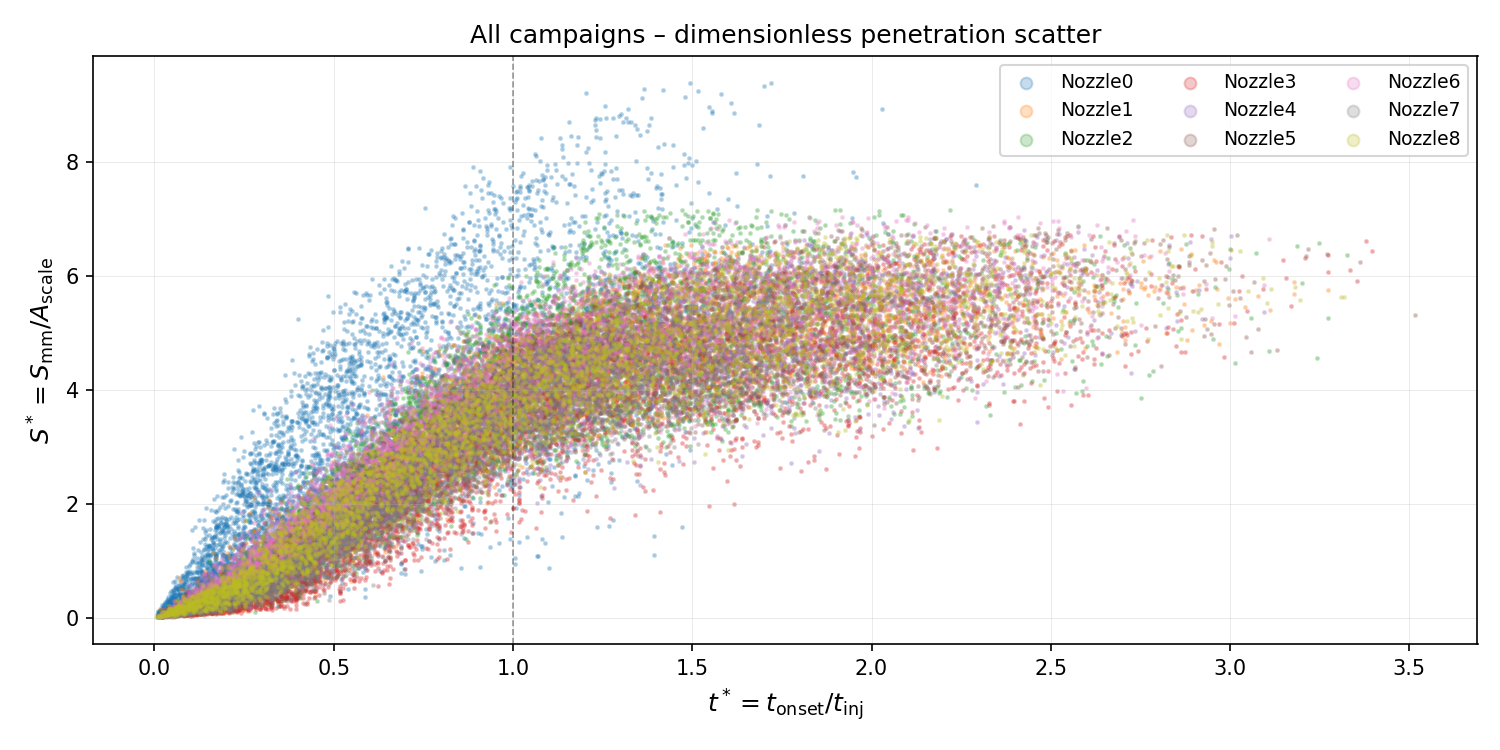
\includegraphics[width=\linewidth]{images/residual_family_head_20260608/injector_scatter_all_nozzles.png}
\end{minipage}
\caption{Why Nozzle0 is out-of-design-family (archived study). Left: normalized early-time penetration response of Nozzle0 ($\approx$2.5$\times$ the modified nozzles and never crossing below it). Right: the full scatter separates Nozzle0's early-time branch, which the frozen trunk never represented.}
\label{fig:injector-comparison}
\label{fig:injector-scatter}
\end{figure}

\begin{figure}[t]
\centering
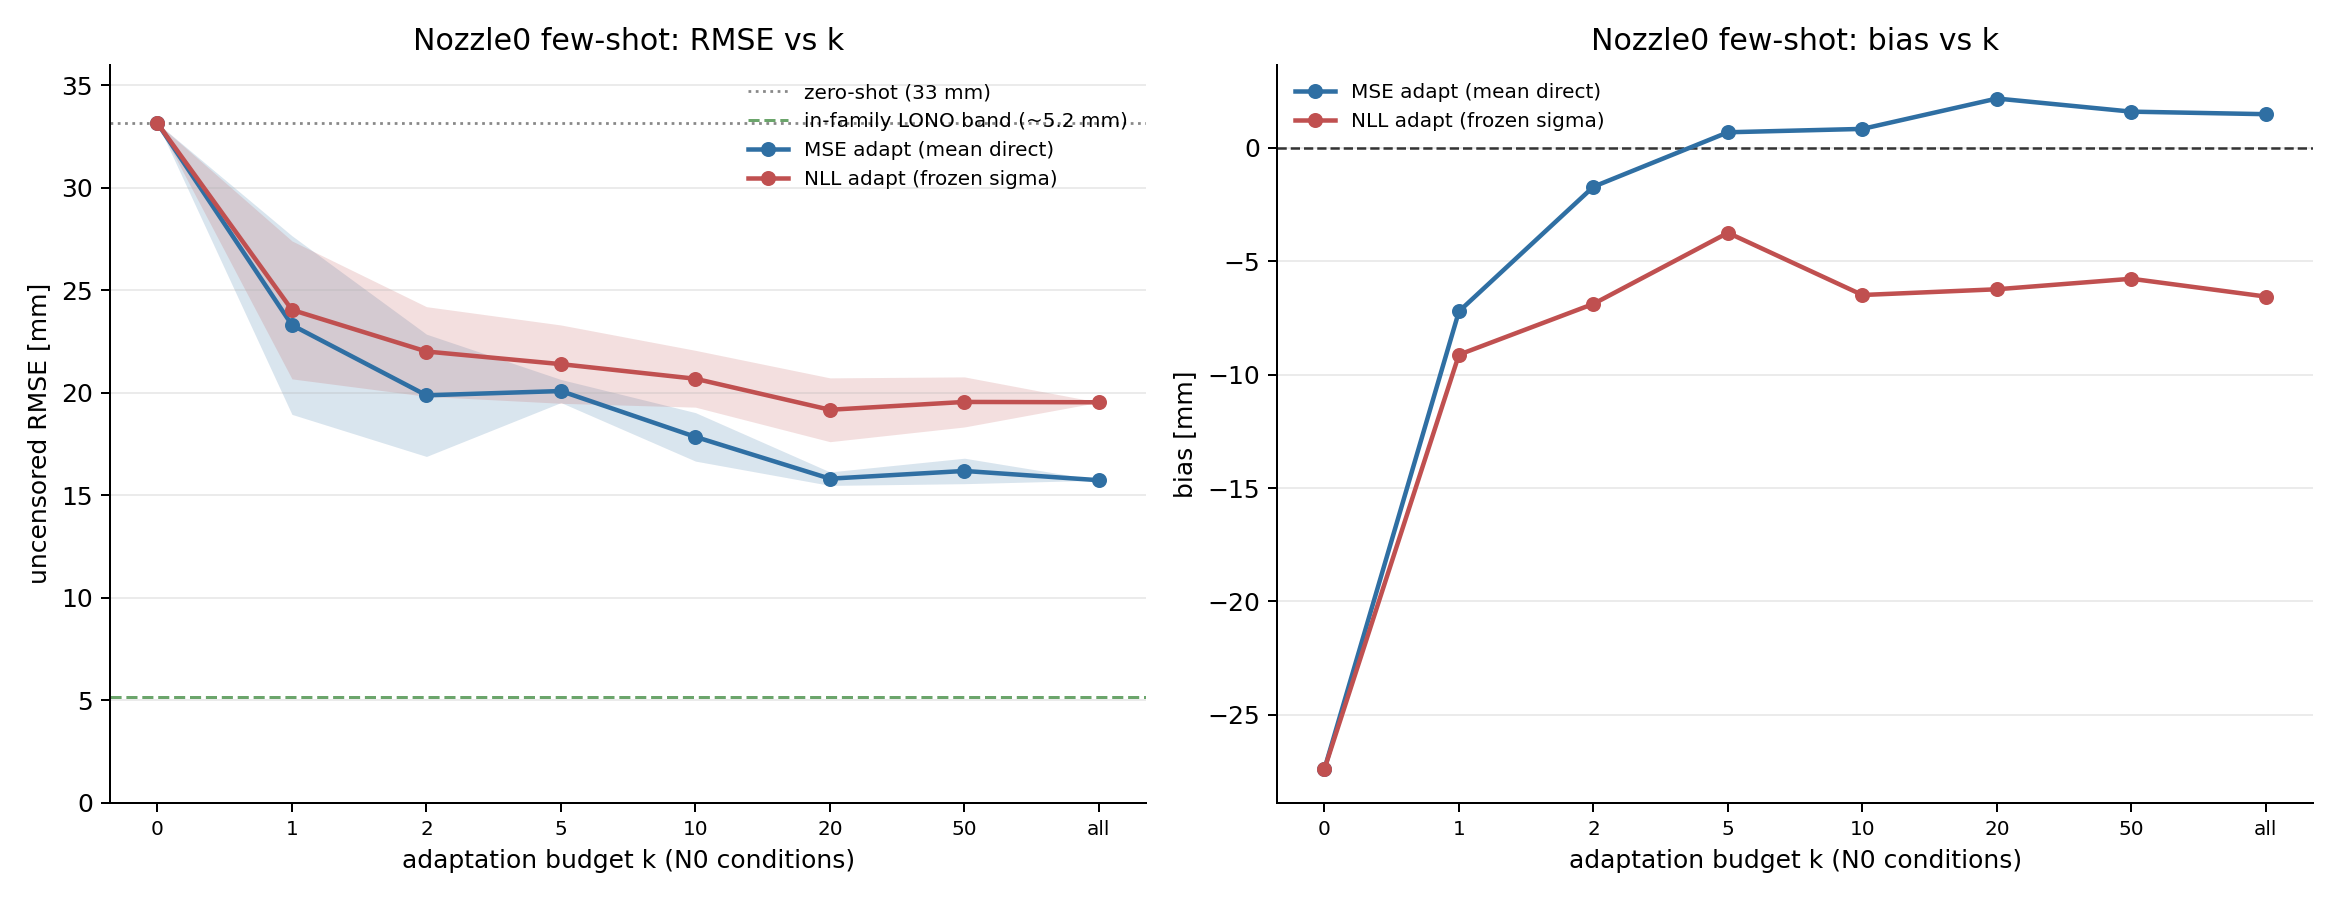
\includegraphics[width=0.62\linewidth]{images/residual_family_head_20260608/n0_fewshot_adaptation_curve.png}
\caption{Archived Nozzle0 few-shot adaptation of the frozen-trunk residual head. Uncensored RMSE versus the number of adapted N0 conditions $k$, for the MSE fine-tune (mean, unthrottled) and the NLL fine-tune (throttled by the frozen variance head). Both plateau far above the $\approx\SI{5}{mm}$ in-family LONO band: delta-only adaptation removes the bias but cannot close the spread.}
\label{fig:n0-fewshot}
\end{figure}

\FloatBarrier
